%%%%%%%%%%%%%%%%%%%%%%%%%%%%%%%%%%%%%%%%%%%%%%%%%%%%%%%%%%%%%%%%%%%%%%%%%%%%%%%%%%%%%%%%%%%%%%%%%%%%%%
% Apuntes de la asignatura Análisis de Fourier
%
% Autores: Andrés Herrera Poyatos (https://github.com/andreshp)
%          Juan Luis Suárez Díaz (https://github.com/jlsuarezdiaz)
%%%%%%%%%%%%%%%%%%%%%%%%%%%%%%%%%%%%%%%%%%%%%%%%%%%%%%%%%%%%%%%%%%%%%%%%%%%%%%%%%%%%%%%%%%%%%%%%%%%%%%

%-----------------------------------------------------------------------------------------------------
%	INCLUSIÓN DE PAQUETES BÁSICOS
%-----------------------------------------------------------------------------------------------------

\documentclass{article}

% Utiliza el paquete de español.
\usepackage{spanish}
% Utiliza la plantilla para reports.
\usepackage{template}

%-----------------------------------------------------------------------------------------------------
%	OTROS PAQUETES
%-----------------------------------------------------------------------------------------------------

\usepackage{mathematics}
\usepackage{physics}
\usepackage{csquotes}
\usepackage{algorithm}
\usepackage{algorithmic}
\usepackage{caption}

% Archivo de traducción
\floatname{algorithm}{Algoritmo}
\renewcommand{\listalgorithmname}{Lista de algoritmos}
\renewcommand{\algorithmicrequire}{\textbf{Entrada:}}
\renewcommand{\algorithmicensure}{\textbf{Salida:}}



\DeclareMathOperator*{\argmin}{arg\,min}
\DeclareMathOperator*{\argmax}{arg\,m \acute ax}

%-----------------------------------------------------------------------------------------------------
% CONFIGURACIÓN DE TABLAS
%-----------------------------------------------------------------------------------------------------

\usepackage{array}

\newcolumntype{L}[1]{>{\raggedright\let\newline\\\arraybackslash\hspace{0pt}}m{#1}}
\newcolumntype{C}[1]{>{\centering\let\newline\\\arraybackslash\hspace{0pt}}m{#1}}
\newcolumntype{R}[1]{>{\raggedleft\let\newline\\\arraybackslash\hspace{0pt}}m{#1}}

%-----------------------------------------------
% BIBLIOGRAPHY
%-----------------------------------------------

\usepackage[
backend=biber
]{biblatex}

\addbibresource{fourier.bib}

%-----------------------------------------------------------------------------------------------------
%	LICENCIA
%-----------------------------------------------------------------------------------------------------

\usepackage[
    type={CC},
    modifier={by},
    version={4.0},
]{doclicense}

%-----------------------------------------------------------------------------------------------------
%	PORTADA
%-----------------------------------------------------------------------------------------------------

\usepackage{title1}

%-----------------------------------------------------------------------------------------------------
%	DATOS DEL DOCUMENTO
%-----------------------------------------------------------------------------------------------------

\newcommand{\doctitle}{Transformada de Fourier Discreta}
\newcommand{\docsubtitle}{}
\newcommand{\docdate}{\date}
\newcommand{\subject}{Análisis de Fourier}
\newcommand{\docauthor}{Marina Estévez \\ Andrés Herrera \\ David Moya \\ Santiago Navarro \\ Adrián Segura \\ Juan Luis Suárez}
\newcommand{\docaddress}{}
\newcommand{\docemail}{}
\newcommand{\docrhead}{Transformada de Fourier Discreta}
\newcommand{\doclhead}{Análisis de Fourier}


%-----------------------------------------------------------------------------------------------------
%	RESUMEN
%-----------------------------------------------------------------------------------------------------

% Resumen del documento. Va en la portada.
% Puedes también dejarlo vacío, en cuyo caso no aparece en la portada.
\newcommand{\docabstract}{}
%\newcommand{\docabstract}{En este texto puedes incluir un resumen del documento. Este informa al lector sobre el contenido del texto, indicando el objetivo del mismo y qué se puede aprender de él.}


% Adds the \pod command, which is \pmod without space:
% https://tex.stackexchange.com/questions/39221/removing-extra-space-with-pmod-command
\renewcommand{\pod}[1]{\allowbreak\mathchoice
  {\if@display \mkern 18mu\else \mkern 8mu\fi (#1)}
  {\if@display \mkern 18mu\else \mkern 8mu\fi (#1)}
  {\mkern4mu(#1)}
  {\mkern4mu(#1)}
}

\begin{document}

\hypersetup{pageanchor=false}
\maketitle
\hypersetup{pageanchor=true}

%-----------------------------------------------------------------------------------------------------
%	ÍNDICE
%-----------------------------------------------------------------------------------------------------

% Profundidad del Índice:
\setcounter{tocdepth}{2}

\newpage
\tableofcontents
\vspace*{\fill}
\doclicenseThis
\newpage

%-----------------------------------------------------------------------------------------------------
%	SECCIÓN 1
%-----------------------------------------------------------------------------------------------------

\section{Introducción}
El análisis de Fourier es el prototipo de rama de las matemáticas que tiene innumerables aplicaciones en otras áreas de la ciencia y de la ingeniería. Desde el tratado de Fourier que tituló con “Théorie Analytique de la Chaleur” (Teoría Analítica del Calor) \cite{fourier}, sus desarrollos se han empleado en ecuaciones en derivadas parciales, análisis armónico, teoría de números y geometría entre otras. No obstante, la versión discreta del análisis de Fourier también juega un papel fundamental en otras disciplinas. Una de ellas es el tratamiento de señales digitales y de imágenes, siendo la transformada de Fourier parte esencial de los algoritmos de compresión usados en la actualidad. La transformada de Fourier también interviene a la hora de acelerar múltiples algoritmos y es por ello considerada una de las herramientas más útiles de la informática teórica.

En este trabajo desarrollamos la Transformada de Fourier Discreta (DFT) y profundizamos en algunas de sus aplicaciones en la teoría de señales y la informática teórica. Esta transformada se desarrolla a partir de la necesidad de los ingenieros de tratar señales, que se generan a partir de un proceso de muestreo de una función típicamente continua. El proceso de discretización suele ser la forma más fácil de aproximar estas señales, evaluándolas en tantos puntos como sea necesario para reconstruir poder reconstruir la señal en el intervalo donde se esté trabajando. La ventaja principal de esta discretización es que, al trabajar en un número finito de puntos, es relativamente sencillo tratar la señal en un ordenador. 

%Nótese aquí que no vamos por tanto a tratar la transformada de Fourier en tiempo discreto (DTFT, Discrete-time Fourier transform), en la que también existe este concepto de discretización pero se hace en una partición con un número infinito de elementos, lo cual hace que no podamos escribir tan cómodamente la notación matricial que vamos a presentar.

En el desarrollo del análisis de Fourier discreto encontraremos un paralelismo evidente con los resultados obtenidos en el caso continuo. No obstante, debido a la naturaleza discreta de la teoría, no hay teoremas que hablen de convergencia o del comportamiento de la transformada en el infinito. Es más, muchos de los conceptos o resultados que en el caso continuo cuentan con una demostración larga y costosa son más sencillos en este ámbito. No obstante, aunque la teoría se simplifique en el análisis discreto, muchas de las aplicaciones de estos resultados son realmente profundas y han supuesto un gran avance para la ciencia en todo su conjunto. El desarrollo de esta área es comparada por varios autores como poseedora de un impacto similar al del desarrollo del cálculo de Newton.

Este trabajo en dos partes principales. La primera parte (Sección \ref{sec:dft} y \ref{sec:dft:2}) consiste en un análisis teórico de la Transformada de Fourier Discreta. En la Sección \ref{sec:dft} definiremos la Transformada de Fourier Discreta unidimensional y estudiaremos sus propiedades, prestando especial interés al Teorema de Inversión, es decir, a recuperar la función a partir de su transformada. También veremos el concepto de convolución en este ambiente. En la Sección \ref{sec:dft:2} se generaliza la Transformada de Fourier Discreta a dos dimensiones. Estas secciones nos proporcionarán un soporte teórico para desarrollar las aplicaciones que se estudian en la segunda mitad del trabajo.  Concretamente, en la Sección \ref{sec:fft} se introduce una serie de algoritmos conocidos como Transformadas de Fourier Rápidas que permiten calcular la transformada discreta de forma eficiente. Estos algoritmos se ejecutan billones de veces cada día. En palabras del investigador G. Strang en 1993, ``La Transformada de Fourier Rápida -- el algoritmo más importante de la historia''. Llegados a este punto cabe reseñar que en la más reciente historia del análisis numérico se adjudica a Carl Friedrich Gauss un algoritmo similar al que presentamos para el cómputo de coeficientes de una serie de Fourier finita. Las primeras evidencias del trabajo de Gauss en este campo se encontraron de forma póstuma en una serie de manuscritos que no se publicaron y que datan de 1805. En la Sección \ref{sec:quantum} se estudia la Transformada de Fourier Cuántica y su aplicación en la computación cuántica para factorizar números enteros mediante el Algoritmo de Shor. Cabe destacar que Shor ganó el premio G\"odel por la publicación de este algoritmo. Finalmente en la Sección \ref{sec:sonido} se introduce el concepto de señal usado por los ingenieros y se relaciona éste con la Transformada de Fourier Discreta.

%Y es que el hecho de que esta rama de las matemáticas tenga ese impacto en nuestro mundo, radica en la necesidad de tener algoritmos rápidos para el cálculo explícito de la transformada. En este sentido y antes de meternos de lleno en el tratamiento de señales, tenemos las partes de transformada de Fourier rápida y de transformada de Fourier cuántica. 



%Like mathematics, computer science will be somewhat different from the other sciences, in that it deals with artificial laws that can be proved, instead of natural laws that are never known with certainty. – Donald Knuth

\section{Transformada de Fourier Discreta} \label{sec:dft}

La Transformada de Fourier Discreta es una herramienta matemática muy usada en ingeniería y computación. Puede definirse, como veremos, partiendo de la Transformada de Fourier continua. Además, tiene propiedades muy importantes análogas a las del caso continuo \cite{bachmann2012fourier}.

Sea $f \in L_1(\R)$. Recordemos que la transformada de Fourier de $f$ viene dada por
\begin{equation} \label{eq:ft}
\widehat{f}(\omega)=\int_{-\infty}^\infty e^{-i\omega t}f(t)\diff t
\end{equation}
para todo $\omega \in \mathbb{R}$. Como nuestra función está en $L_1(\R)$ esto nos dice que $f(t)$ tiende a $0$ cuando $|t|$ diverge. En consecuencia, es claro que la integral en un intervalo compacto $[a,b]$ para $a<0$, $b>0$ y $|a|, |b|$ suficientemente grandes se aproxima al valor de la integral \eqref{eq:ft}, esto es,
 \begin{equation} \label{eq:ft:ab}
 \widehat{f}(\omega) \approx \int_{a}^b e^{-i\omega t}f(t)\diff t.
 \end{equation}
 La idea para definir la Transformada de Fourier Discreta viene dada por aproximar \eqref{eq:ft:ab} por métodos numéricos, concretamente, mediante una suma de Riemann de $f$ en $[a,b]$. Es decir, realizamos la aproximación
 %Si hacemos una partición para tener un proceso similar al de las sumas de Riemann a la hora de construir su integral nos encontramos con el problema de que necesitamos un intervalo compacto y es por esto la discusión anterior. Por tanto lo que haremos es:
 \begin{equation} \label{eq:ft:d}
 \widehat{f}(\omega) \approx \sum_{k=0}^{N-1}f(t_k)e^{-i\omega t_k} (t_{k+1} - t_{k}),
 \end{equation}
 con $\{a=t_0<t_1<...<t_{N-1}=b\}$, una partición con espaciado uniforme del intervalo $[a,b]$ y de cardinal $N$. Para $\Delta t =(b-a)/ N$ tenemos por tanto que $t_k=a+k\Delta t$, $k \in \{0,1, \ldots, N-1\}$. Llamando $\phi$ a la aproximación de $\widehat{f}$ dada en \eqref{eq:ft:d} obtenemos 
 \[
 \phi(\omega)=\sum_{k=0}^{N-1} f(t_k)e^{-i\omega t_k }\Delta t=e^{i\omega a}\sum_{k=0}^{N-1} f(t_k)e^{-i\omega k (b-a)/N  }\Delta t.
 \]
 Por último llamando $\omega_n=2\pi n / (b-a)$ tenemos que 
 \[
 \phi(\omega_n)=e^{i\omega_n a}\sum_{k=0}^{N-1}f(t_k)e^{-i2\pi nk/N}\Delta t,
 \]
 lo que nos da pie a hacer la siguiente definición.
 
 Dada $f\colon\R \longrightarrow \C$ una función se define la \emph{Transformada de Fourier Discreta de $f$} como la aplicación $Df\colon\Z \longrightarrow \C$ donde, 
 \[
 Df(n) = \sum_{k=0}^{N-1}f(t_k)e^{-i2\pi nk/N},
 \]
 o para simplificar, si llamamos $\zeta_N=e^{2\pi i/N}$, es decir usamos las raíces de la unidad a la hora de escribir nuestra fórmula, entonces obtenemos
 \[
Df(n) = \sum_{k=0}^{N-1}f(t_k)\zeta_N^{-nk}.
 \]

En otros textos por cuestiones de normalización podemos encontrar esta misma definición normalizando por $1/N$ o $1/ \sqrt{N}$. Nosotros trabajaremos con la Transformada de Fourier Discreta sin normalizar salvo en el caso de la Transformada de Fourier Cuántica (véase la Sección \ref{sec:quantum:qft}). Cuando no haya riesgo de confusión escribiremos $\zeta$ en lugar de $\zeta_N$.

Vamos a tratar ahora de dar un enfoque más discreto a la definición. Como estamos trabajando con un número finito de términos de la función $f$ , podemos obviar por un momento que está definida en todo $\R$. Por tanto, supondremos que $f$ está definida en el conjunto $\{ 0,1,\dots ,N-1 \}$. Es decir, vemos a la función $f$ como una $n$-upla de números complejos, esto es, $(f(0),f(1),\dots ,f(N-1)) \in \C ^N$. También podemos ver la función $f$ definida en el grupo cíclico de orden N, que denotaremos $\Z _N = \Z / N \Z $.
Así, la función $f$ quedaría del siguiente modo:
\[
    \begin{array}{rccl}
        f \colon & \Z _N & \longrightarrow & \C \\
        & k+N\Z & \longmapsto & f(k).
    \end{array}
\]
También se puede ver a la función $f$ como una función $N$-periódica definida en $\Z$, esto es, $f(k+nN) = f(k)$ para todo $k \in \{0,1,2, \dots ,N-1\}$, $n \in \Z$.
\begin{definition}
    Supongamos que el conjunto finito $\Z _N$ está dotado de la medida discreta, es decir, todos los subconjuntos de $\Z _N$ son medibles y la medida de cada subconjunto es el número de elementos que tiene el subconjunto. Por tanto, como $\Z _N$ es finito, cada función definida en $\Z_N$ es integrable. Así, $L_1 (\Z _N ) = L_2 (\Z _N ) = \C ^N$ es el conjunto formado por todas las funciones del tipo $f \, : \Z _N \rightarrow \C $. La Transformada de Fourier Discreta (DFT) de $f \colon \Z _N \to \C $ es la aplicación $D_N f \colon \Z_N \to \C$ dada por
    \begin{equation}
        D_N f(n) = \sum_{k=0}^{N-1}f(k)e^{-2\pi ink/N}
        \label{def:DFT}
    \end{equation}
    para todo $n \in \Z_N$. %Además, como $Df$ es $N$-periódica podemos verla también definida en $\Z _N$.
    Se define el operador de la Transformada de Fourier Discreta como
\[
    \begin{array}{rccl}
        F\colon & L_1( \Z _N) & \longrightarrow & L_1( \Z _N) \\
        & f & \longmapsto & D_N f
    \end{array}
\]
Cuando no haya riesgo de confusión escribiremos $D f$ en lugar de $D_N f$.
\end{definition}

\subsection{Forma Matricial}\label{sec:matrix}
Partiendo de la definición de Transformada de Fourier Discreta de una función $f$ y de cardinal $N$,
\[
Df(n)=\sum_{k=0}^{N-1}f(t_k) \zeta^{-nk}, \text{ con }  \zeta=e^{2\pi i/N},
\]
y teniendo en cuenta que $f,Df\in L_{1}(\mathbb{Z}_{N})$ podemos ver la función $f$ y su trasformada $Df$ como vectores, esto es,
\[
Df=\begin{pmatrix}
Df(0)\\ \vdots\\Df(N-1)\\
\end{pmatrix}
, \quad
f=\begin{pmatrix}
f(0)\\ \vdots\\f(N-1)\\
\end{pmatrix}.
\]
%Nótese que hemos considerado ahora una escritura por columnas en vista a tener una expresión matricial lo más simple posible.
Definimos la matriz
\[
M_{N}=\begin{pmatrix}
1      &  1             & 1               & \cdots & 1 \\
1      & \zeta^{-1}     & \zeta^{-2}      & \cdots & \zeta^{-(N-1)} \\
1      & \zeta^{-2}     & \zeta^{-4}      & \cdots & \zeta^{-2(N-1)} \\
\vdots & \vdots         & \vdots          & \ddots & \vdots\\
1      & \zeta^{-(N-1)} & \zeta^{-2(N-1)} & \cdots & \zeta^{-(N-1)^2} \\
\end{pmatrix}.
\]
 A partir de la definición de DFT es fácil ver que $Df=M_{N}\,f$. En vista de esto resulta evidente que el operador de la Transformada de Fourier Discreta es lineal por obtenerse como producto por una matriz. Teniendo en cuenta que $\zeta^N = 1$ podemos simplificar la expresión anterior, obteniendo
 %Y al igual que en esta podemos simplificar la expresión de $M_{N}$ en términos de $ \zeta=e^{2\pi i/N}$, la primera raíz N-ésima de la unidad (esta forma es más útil de manejar a la hora de hacer ejemplos concretos, como veremos), como sigue
\begin{equation} \label{eq:mn}
M_{N}=\begin{pmatrix}
1&1&1&\dots&1 \\
1&\overline{ \zeta}&\overline{ \zeta}^{2}&\cdots&\overline{ \zeta}^{N-1}\\
1&\overline{ \zeta}^{2}&\overline{ \zeta}^{4}&\cdots&\overline{ \zeta}^{N-2}\\
\vdots&\vdots&\vdots&\ddots&\vdots\\
1&\overline{ \zeta}^{N-1}&\overline{ \zeta}^{N-2}&\cdots&\overline{ \zeta}\\
\end{pmatrix}.
\end{equation}

Nótese que $M_N$ es una matriz de Vardenmonde. Recordemos que la estructura habitual de una matriz de ese tipo es
\[
V(x_{0},\dots,x_{n})=\begin{pmatrix}
1&x_{0}&x_{0}^{2}&\dots&x_{0}^{n} \\
1&x_{1}&x_{1}^{2}&\dots&x_{1}^{n} \\
\vdots&\vdots&\vdots&\ddots&\vdots\\
1&x_{n}&x_{n}^{2}&\dots&x_{n}^{n} \\
\end{pmatrix}.
\]

En nuestro caso la matriz $M_N$ responde a esta estructura llamando $x_k=\overline{\zeta}^k$ para todo $k \in \{0, \dots, N-1\}$.% y dándonos cuenta de que, como estamos trabajando módulo $N$, los exponentes se simplifican para dar lugar a la matriz $M_N$.  
Recordemos que el determinante de una matriz de Vandermonde es $\prod_{i>j}(x_i-x_j)$. Aplicando esta fórmula a $M_N$ obtenemos
\[
\det(M_N)=\prod_{i>j}(\zeta^{-i}-\zeta^{-j}),
\]
que es distinto de $0$ ya que $\zeta^{-i} \ne \zeta^{-j}$ para todo $i \ne j$.

Vamos a probar ahora algunas propiedades de la transformada discreta, que son análogas a algunas propiedades de la transformada continua.
\begin{proposition} \label{prop:dft:prop}
Fijemos $j \in \Z$ y sea $f\colon\Z_N \longrightarrow \C$. Se verifican las siguientes afirmaciones:
\begin{enumerate}
    \item La DFT de $f(n-j)$ es $Df(n) \zeta^{-jn}$.
    \item La DFT de $f(n) \zeta^{jn}$ es $Df(n-j)$. \label{item:dft:b}
    \item La DFT de $f(n)\cos(2\pi jn/N)$ es $(Df(n-j)+Df(n+j)) / 2$.
\end{enumerate}
\end{proposition}

\begin{proof}~
\begin{enumerate}
    \item Sea $g(n)=f(n-j)$. Tenemos que
    \[
    Dg(n)=\sum_{k=0}^{N-1}g(k)\zeta^{-kn}=\sum_{k=0}^{N-1}f(k-j)\zeta^{-kn}.
    \]
    Si hacemos el cambio $m=k-j$ y separamos la sumatoria obtenemos
    \begin{align*}
    Dg(n) & =\sum_{m=-j}^{-1}f(m)\zeta^{-(m+j)n}+\sum_{m=0}^{N-1-j}f(m)\zeta^{-(m+j)n} \\
    & =\sum_{m=N-j}^{N-1}f(m)\zeta^{-(m+j)n}+\sum_{m=0}^{N-1-j}f(m)\zeta^{-(m+j)n} \\
    & =\left(\sum_{m=0}^{N-1}f(m)\zeta^{-mn}\right)\zeta^{-jn} =Df(n)\zeta^{-jn},
    \end{align*}
    donde en la segunda igualdad hemos usado que $f$ es N-periódica y, por tanto, sumar desde $-j$ hasta $-1$ es lo mismo que sumar desde $N-j$ hasta $N-1$.
    \item La transformada de $g(n) = f(n)\zeta^{jn}$ es 
    \[
    Dg(n) = \sum_{k=0}^{N-1}f(k)\zeta^{jk}\zeta^{-kn}=\sum_{k=0}^{N-1}f(k)\zeta^{-k(n-j)}=Df(n-j).
    \]
    \item Aplicando la definición del coseno complejo obtenemos
    \[
    g(n) = f(n)\cos(2\pi jn/N)=\frac{1}{2}\left(f(n)\zeta^{jn}+f(n)\zeta^{-jn}\right).
    \]
    Y ahora aplicando \ref{item:dft:b} deducimos que 
    \[
    Dg(n) = \frac{1}{2}Df(n-j)+\frac{1}{2}Df(n+j). \qedhere
    \]
\end{enumerate}
\end{proof}

Por último antes de finalizar esta sección introductoria vamos a hacer algún ejemplo de cálculo explícito de una DFT.

\begin{ex}
Consideremos una función constante: sea $f\colon Z_4 \longrightarrow \C$, $f\equiv(1,1,1,1)$. Hallar su Transformada de Fourier Discreta.

Solución:
Hemos elegido hacerlo en $Z_4$ por la simplicidad de escritura de las raíces cuartas de la unidad. Así obtenemos
\[
Df=M_{4}f=\begin{pmatrix}
1&1&1&1 \\
1&-i&-1&i\\
1&-1&1&-1\\
1&i&-1&-i\\
\end{pmatrix}
\,
\begin{pmatrix}
1\\1\\1\\1\\
\end{pmatrix}=
\begin{pmatrix}
4\\0\\0\\0\\
\end{pmatrix} \qedhere
\]
\end{ex}

\begin{ex} \label{ex:g_muchas_is}
Sea $g=(1,i,i^2,i^3)=(1,i,-1,-i)$, que se podría ver como la discretización de $g(t)=i^t$ considerando el espacio $\Z_4$.

Esta función cumple que $g(k)=1\cdot i^{k}=f(k)e^{2\pi ik/4}$ para todo $k\in\{0,1,2,3\}$ y, por tanto, podemos aplicar la propiedad \ref{item:dft:b} de la Proposición \ref{prop:dft:prop} para obtener

\[
Dg(0)=Df(0-1)=Df(3)=0,
\]
\[
Dg(1)=Df(1-1)=Df(0)=4,
\]
\[
Dg(2)=Df(2-1)=Df(1)=0,
\]
\[
Dg(3)=Df(3-1)=Df(2)=0,
\]
donde $f$ es la función definida en el ejemplo anterior.
\end{ex}

\subsection{Teorema de inversión para la DFT}

Vamos a tratar de recuperar $f$ a partir de su Transformada de Fourier Discreta. Para ello, vamos a enunciar y demostrar el Teorema de Inversión para la DFT, que, como veremos, se puede expresar de tres modos distintos. 
Nótese que el espacio $L_1(\Z_N)$ formado por todas las funciones del tipo $f\colon\Z_N \rightarrow \C$ con el producto escalar dado por
\[
    \langle f,g \rangle = \sum_{k=0}^{N-1}f(k)\overline{g(k)}
\]
para todo $f,g \in L_1(\Z _N)$. Este espacio es precisamente $\C^N$ con su producto escalar usual. Por tanto, $L_1(\Z_N)$ es un espacio de Hilbert.
Antes de enunciar y demostrar el Teorema de Inversión en su primera forma, necesitamos un resultado previo.
\begin{lemma} \label{lem:sumroots}
    Sea $N \in \N$ con $N\ge 2$. Consideremos las raíces $N$-ésimas de la unidad dadas por $\zeta^m = e^{2\pi im / N}$ para $m \in \{1,2, \dots , N-1\}$. Entonces
    \begin{equation*}
        \sum_{k=0}^{N-1}\zeta ^k = 0.
    \end{equation*}
\end{lemma}
\begin{proof}
    La idea consiste en ver la sumatoria del enunciado como una serie geométrica y calcular su suma parcial aprovechando que $N\ge 2$. Tenemos que
    \[
        \sum_{k=0}^{N-1}\zeta ^k = \frac{\zeta^N - 1}{\zeta - 1} = 0. \qedhere
        %\sum_{k=0}^{N-1}e^{2\pi imk/N} = \sum_{k=0}^{N-1}\left( e^{2\pi im / N} \right) ^k = S.
    \]
%    Como tenemos que $N\ge 2 \Rightarrow e^{2\pi im / N} \neq 1$, entonces, haciendo la suma parcial de la serie geométrica, nos queda:
%    \[
%        S = \frac{\left( e^{2\pi im / N} \right) ^0 - \left( e^{2\pi im / N} \right) ^N }{1 - e^{2\pi im / N}} = \frac{1 - 1}{1 - e^{2\pi im / N} } = 0 \qedhere
%    \]
\end{proof}

Veamos ahora el Teorema de Inversión.

\begin{theorem}[Teorema de Inversión]\label{thm:inv}
    Sea $f\colon\Z_N \rightarrow \C$, con Transformada de Fourier Discreta dada por
    \[
        Df(n) = \sum_{k=0}^{N-1}f(k)e^{-2\pi ink /N} = \sum_{k=0}^{N-1} f(k)  \zeta ^{-kn},
    \]
    Entonces, se tiene que
    \begin{equation}
        f(n) = \frac{1}{N} \sum_{k=0}^{N-1} Df(k)e^{2\pi ink / N} = \frac{1}{N} \sum_{k=0}^{N-1} Df(k) \zeta ^{kn}.
        \label{eq:inversion2}
    \end{equation}
\end{theorem}
\begin{proof}
    Para demostrar este teorema, la idea será partir de $\sum_{k=0}^{N-1} Df(k) \zeta^{nk} / N$ , y probar que es igual a $f(n)$ usando el Lema \ref{lem:sumroots}. En efecto, tenemos que 
    \begin{align*}
         \frac{1}{N} \sum_{k=0}^{N-1} Df(k) \zeta ^{kn} & = \frac{1}{N} \sum_{k=0}^{N-1} \left( \sum_{j=0}^{N-1} f(j)  \zeta ^{-kj} \right)  \zeta ^{kn} \\
            & = \frac{1}{N} \sum_{j=0}^{N-1} f(j) \left( \sum_{k=0}^{N-1}  \zeta ^{k(n-j)} \right).
    \end{align*}
    Observando la última expresión, vemos que para $n=j$ se tiene que $\sum_{k=0}^{N-1}  \zeta ^{k(n-j)} = \sum_{k=0}^{N-1} 1 = N$, mientras que para $n \neq j$, denotando $n-j = m$, se tiene que
    \[
        \sum_{k=0}^{N-1}  \zeta ^{k(n-j)} = \sum_{k=0}^{N-1} \left(  \zeta ^{n-j} \right) ^k = \sum_{k=0}^{N-1} \left(  \zeta ^{m} \right) ^k = 0,
    \]
    donde hemos usado el Lema \ref{lem:sumroots} en la última igualdad. Así, finalmente obtenemos
    \[
        \frac{1}{N} \sum_{k=0}^{N-1} Df(k)e^{2\pi ink / N} = \frac{1}{N}f(n)N = f(n). \qedhere
    \]
\end{proof} 
De este Teorema de Inversión deducimos que la Transformada de Fourier Discreta (DFT) es una biyección lineal.

\begin{definition}
    Definimos para cada $j \in \{0,\dots,N-1\}$ la función $\zeta_j \colon \Z_N \to \C$ dada por $\zeta_j(m)= \zeta^{-jm}$ para todo $m \in \{0,1,\ldots,N-1\}$.

    Al igual que con $f$ y $Df$ podemos ver esta familia de funciones como los vectores
    \[ \zeta_j = \left( 1, \zeta^{-j}, \zeta^{-2j}, \dots , \zeta^{-(N-1)j} \right).\]
\end{definition}

\begin{lemma}
    El conjunto $\{ \zeta_j/\sqrt{N} : j=0,\dots,N-1\}$ es una base ortonormal de $L_1(\mathbb{Z}_N).$
\end{lemma}
\begin{proof}
  Puesto que $L_1(\mathbb{Z}_N)$ es un espacio de dimensión $N$ basta probar que para cualquier pareja $k,j \in \{0,1,\ldots,N-1\}$ se verifica
  \[
  \langle \frac{1}{\sqrt{N}} \zeta_j,\frac{1}{\sqrt{N}} \zeta_k\rangle=\delta_{kj}.
  \]
  En efecto, nótese que
  \[
  \langle \frac{1}{\sqrt{N}} \zeta_j,\frac{1}{\sqrt{N}} \zeta_k\rangle=\frac{1}{N}\langle \zeta_j, \zeta_k\rangle=\frac{1}{N}\sum_{n=0}^{N-1} \zeta_j(n)\overline{ \zeta_k(n)}=\frac{1}{N}\sum_{n=0}^{N-1} \zeta^{(k-j)n}.
  \]
  Si $j=k$ tenemos que,
  \[\frac{1}{N}\sum_{n=0}^{N-1} \zeta^{(k-j)n}=\frac{1}{N}\sum_{n=0}^{N-1} \zeta^{0}=1.\]
  Si $j\neq k$ entonces por el Lemma \ref{lem:sumroots} para $m=k-j$ obtenemos
  \[\frac{1}{N}\sum_{n=0}^{N-1}\zeta^{(k-j)n}=\frac{1}{N}\sum_{n=0}^{d-1}\left(\zeta^m\right)^n=0. \qedhere\]
\end{proof}

Veamos como este resultado permite demostrar el Teorema de Inversión de manera alternativa. Puesto que  $\{ \zeta_j/\sqrt{N} : j\in\{0,\dots,N-1\}\}$ es una base ortonormal de $L_1(\Z_N)$ es fácil comprobar que el conjunto $\{\overline{ \zeta_j}/\sqrt{N} : j\in\{0,\dots,N-1\}\}$ también lo es.
De esta manera cada $f\in L_1(\mathbb{Z}_N)$ se puede expresar de la forma
\[f=\sum_{j=0}^{N-1}\langle f,\frac{1}{\sqrt{N}}\overline{ \zeta_j}\rangle \frac{1}{\sqrt{N}}\overline{ \zeta_j}.\]
Además, tenemos que
\[\langle f,\frac{1}{\sqrt{N}}\overline{ \zeta_j}\rangle=\frac{1}{\sqrt{N}}\sum_{m=0}^{N-1}f(m) \zeta^{-jm}=\frac{1}{\sqrt{N}}Df(j).\]
Por lo tanto, 
\[f=\sum_{j=0}^{N-1} \frac{1}{\sqrt{N}}Df(j)\frac{1}{\sqrt{N}}\overline{ \zeta_j}=\frac{1}{N}\sum_{j=0}^{N-1}Df(j)\overline{ \zeta_j}.\]

Que es justo el mismo resultado que obtuvimos por el Teorema de Inversión.

\begin{proposition}
    Sean $f,g \in L_2(\Z_N)$. Entonces, se verifican las igualdades de Parseval:
    \begin{align*}
\sum_{k=0}^{N-1}f(k)\overline{g(k)} =\, &\frac{1}{N} \sum_{k=0}^{N-1}Df(k)\overline{Dg(k)},\\
\sum_{k=0}^{N-1} |f(k)|^2 = \, &\frac{1}{N} \sum_{k=0}^{N-1} |Df(k)|^2 .
    \end{align*}
\end{proposition}
\begin{proof}
%        \[
%%            f(n) = \frac{1}{N} \sum_{k=0}^{N-1}Df(k)\overline{ \zeta_n(k)}
%        \]
%        Teniendo en cuenta esto y denotando:
%        \[
%            \delta_{kj} =\left\{ \begin{array}{cc}
%                 0 & \hbox{si } k \neq j \\
%%                 &  \\
%                 1 & \hbox{si } k = j \\
%            \end{array}
%            \right.
%        \]
    Aplicando el Teorema de Inversión deducimos que
        \begin{align*}
            \sum_{n=0}^{N-1}f(n)\overline{g(n)}  & = \sum_{n=0}^{N-1}\left( \frac{1}{N} \sum_{k=0}^{N-1} Df(k)\overline{ \zeta_n(k)} \right) \left( \frac{1}{N} \overline{\sum_{j=0}^{N-1} Dg(j)\overline{ \zeta_n(j)} } \right) \\
             & = \frac{1}{N} \sum_{j=0}^{N-1} \overline{Dg(j)} \sum_{k=0}^{N-1} Df(k) \frac{1}{N} \sum_{n=0}^{N-1}\overline{ \zeta_n(k)} \zeta_n(j) \\
             & = \frac{1}{N} \sum_{j=0}^{N-1} \sum_{k=0}^{N-1} Df(k) \overline{Dg(j)} \delta_{kj} \\
             & = \frac{1}{N} \sum_{j=0}^{N-1} Df(j) \overline{Dg(j)}.
        \end{align*}
    Tomando $g = f$ en la desigualdad que acabamos de demostrar obtenemos
        \begin{align*}
            \sum_{k=0}^{N-1} |f(k)|^2 = \sum_{k=0}^{N-1}f(k)\overline{f(k)} & = \frac{1}{N} \sum_{k=0}^{N-1}Df(k)\overline{Df(k)} = \frac{1}{N} \sum_{k=0}^{N-1} |Df(k)|^2.  \qedhere
        \end{align*}
\end{proof}

\begin{comment}
Usando la notación $ \zeta = e^{\frac{2\pi i}{N}}$, $Df = M_N f$, tenemos:
\[
    M_{N} = \begin{pmatrix}
    1 & 1 & 1 & \dots & 1 \\
    1 & \overline{\zeta} & \overline{\zeta}^{2} & \cdots & \overline{\zeta}^{N-1} \\
    1 & \overline{\zeta}^{2} & \overline{\zeta}^{4} & \cdots & \overline{\zeta}^{N-2} \\
    \vdots & \vdots & \vdots & \ddots & \vdots \\
    1 & \overline{\zeta}^{N-1} & \overline{\zeta}^{N-2} & \cdots & \overline{\zeta} \\
    \end{pmatrix}
\]
Recordemos la notación:
\[
     \zeta_j(m) = \left( 1, \overline{ \zeta}^j, \overline{ \zeta}^{2j}, \dots , \overline{ \zeta}^{(N-1)j} \right).
\]
\end{comment}

Otro modo de deducir el Teorema de Inversión consiste en utilizar la inversa de la matriz $M_N$, que se introdujo en \eqref{eq:mn}. 
Los vectores $ \zeta_i / \sqrt{N}$, $i\in\{0, \dots , N-1\}$, en $L_1(\Z_N)$ son las filas de la matriz $\left( 1 / \sqrt{N} \right) M_N = ( \zeta_k (j) ) = (\overline{ \zeta}^{kj} )$, esto es,
\[
    M_{N} = \begin{pmatrix}
     \zeta_0 \\
     \zeta_1 \\
    \vdots \\
     \zeta_{N-1} \\
    \end{pmatrix}.
\]
Se tiene que $ \zeta_k(j) = \overline{ \zeta}^{kj} = \overline{ \zeta}^{jk} =  \zeta_j(k)$. Por tanto, se sigue que la matriz $M_N$ es simétrica, es decir, que coincide con su traspuesta, $M_N = M_N^t$.
\begin{definition}
    Sea $N\in \N$. Consideremos $A = (a_{ij}) $ una matriz de dimensión $N\times N$. Definimos la matriz adjunta de $A$ como
    \[
        A^{\ast} = (\overline{a}_{ji}).
    \]
    Notemos que en el caso de que la matriz $A$ sea simétrica, entonces $A^{\ast} = (\overline{a}_{ji}) = (\overline{a}_{ij}) $
\end{definition}
Teniendo en cuenta que $M_N$ es simétrica, los vectores $ \zeta_i / \sqrt{N}$ son ortonormales y denotando por ${\bf I}$ a la matriz identidad, en este caso de dimensión $N\times N$, se tiene que
\[
    M_N M_N^* = \begin{pmatrix}
    N & 0 & 0 & \dots & 0 \\
    0 & N & 0 & \cdots & 0 \\
    0 & 0 & N & \cdots & 0 \\
    \vdots & \vdots & \vdots & \ddots & \vdots \\
    0 & 0 & 0 & \cdots & N \\
    \end{pmatrix} = N{\bf I}
\]

    Por tanto, despejando la matriz inversa de la expresión anterior y multiplicando a la izquierda por la matriz inversa de $M_N$, que existe pues $M_N$ tiene determinante no nulo, nos queda
\[
    \frac{1}{N}M_N^{\ast} = M_N^{-1}.
\]
Finalmente, como $Df = M_N f$, se obtiene:
\[
    f = M_N^{-1}Df = \frac{1}{N}M_N^{\ast}Df.
\]
Así, acabamos de ver una tercera manera de obtener la inversa de la Transformada de Fourier Discreta.

\begin{corollary} \label{cor:isometria}
    El automorfismo de $\mathbb{C}^N$ cuya matriz respecto de la base usual es $M_N / \sqrt{N}$ es una isometría.
    %La expresión anterior nos dice además que $\frac{M_N}{\sqrt{N}}$ es un operador unitario.
\end{corollary}

\subsection{Convolución}
Una de las propiedades más importantes de una transformada de Fourier es la dualidad que existe entre convolución y producto puntual. Sabemos así que en $L_1(\mathbb{T})$ y $ L_1(\R)$ se verifica: $\widehat{f*g}= \hat{f} \cdot \hat{g}$. Vamos a definir el análogo a la convolución en nuestro contexto y probar la propiedad análoga.

\begin{definition}
Sean $f,g \in L_1(\Z_N)$ se define la convolución de $f$ y $g$ como la función $f \ast g \in L_1(\Z_N)$ dada por
\[
(f\ast g)(k)=\sum_{j=0}^{N-1}f(j)g(k-j)
\]
para todo $k \in Z_N$.
\end{definition}

Nótese la utilidad de trabajar en $Z_N$ para que la definición tenga sentido. Las propiedades básicas de la convolución son las que se listan en  la siguiente proposición.

\begin{proposition}
Sean $f,g,h \in L_1(Z_N)$. Se verifican las siguientes afirmaciones:
\begin{enumerate}
    \item $f\ast g=g\ast f$;
    \item $f\ast (g\ast h)=(f\ast g)\ast h$;
    \item $a(f\ast g)=(af)\ast g$ con $a \in \R$;
    \item $f\ast(g+h)=f\ast g+f\ast h$.
\end{enumerate}
\end{proposition}
\begin{proof}~
\begin{enumerate}
    \item Aprovechando la periodicidad tenemos:
    \begin{align*}
    (f\ast g)(k) & =\sum_{j=0}^{N-1}f(j)g(k-j)=\sum_{m=k}^{k-N+1}f(k-m)g(m) \\ &=\sum_{m=0}^{-(N-1)}f(k-m)g(m)=\sum_{m=0}^{N-1}f(k-m)g(m).
    \end{align*}
    \item Para cada $k \in \Z_N$ tenemos que
    \begin{align*}
    (f \ast g)\ast h (k)& =\sum_{j=0}^{N-1}(f \ast g)(j)h(k-j)=\sum_{j=0}^{N-1}\sum_{\beta=0}^{N-1}f(\beta)g(j-\beta)h(k-j)= \\
    & =\sum_{j=0}^{N-1}\sum_{\gamma=0}^{N-1}f(j)g(\gamma)h(k-j-\gamma)=\sum_{j=0}^{N-1}f(j)g \ast h(k-j)=f \ast (g \ast h)(k)
    \end{align*}
    \item $a(f\ast g)(k)=\displaystyle\sum_{j=0}^{N-1}af(j)g(k-j)=((af)\ast(g))(k)$ 
    \item Para cada $k \in \Z_N$ tenemos que
    \begin{align*}
    f\ast(g+h)(k) & =\displaystyle\sum_{j=0}^{N-1}f(j)(g+h)(k-j)= \sum_{j=0}^{N-1}f(j)(g(k-j)+h(k-j)) \\
     & =\displaystyle\sum_{j=0}^{N-1}f(j)g(k-j)+\sum_{j=0}^{N-1}f(j)h(k-j)=(f\ast g+f\ast h)(k) \qedhere
    \end{align*}
\end{enumerate}
\end{proof}

\begin{theorem}
  Para $f,g \in L_1(\Z_N)$ se verifica que $D(f \ast g)(n)=Df(n)Dg(n)$ para todo $n \in \Z_N$.
\end{theorem}

\begin{proof}
 Sea $n \in \Z_N$. Tenemos que
  \begin{align*}
    D(f\ast g)(n) &= \sum_{k=0}^{N-1}f \ast g(k)e^{-2\pi ikn/N}
    =\sum_{k=0}^{N-1} f \ast g(k)\zeta^{-kn}\\
    &=\sum_{k=0}^{N-1} \left(\sum_{j=0}^{N-1} f(j)g(k-j)\right)\zeta^{-kn}
    =\sum_{j=0}^{N-1}f(j)\left(\sum_{k=0}^{N-1}g(k-j)\zeta^{-kn}\right)\\
    &=\sum_{j=0}^{N-1} f(j)w^{jn}\left(\sum_{k=0}^{N-1}g(k-j)\zeta^{-(k-j)n}\right)
    =Df(n)Dg(n). \qedhere
    \end{align*}    
\end{proof}

Por último recordamos que no existía la unidad para la convolución cuando trabajábamos en $L_1(\R^n)$. En nuestro caso, $L_1(\Z_N)$ si que tenemos una función que actúa como unidad:
\[
e(k)=(1,0,\dots,0),
\]
con la que tenemos simplemente aplicando la definición que $f \ast e=f \quad \forall f \in L_1(Z_N)$. 

\newpage

\section{Transformada de Fourier Discreta Bidimensional} \label{sec:dft:2}

\subsection{Definiciones}

La Transformada de Fourier Discreta bidimensional es una de las más importantes a la hora de aplicaciones en señales de imágenes y vídeos. Podemos encontrar diversa información teórica y acerca de sus aplicaciones en multitud de libros \cite{rao2011fast}. La Transformada de Fourier Discreta en dos dimensiones se define como sigue:
\begin{definition}
    Sean $N_1, N_2 \in \N$. Sean $ \zeta_{N_{1}} = e^{2\pi i / N_1}$ y $ \zeta_{N_{2}} = e^{2\pi i / N_2}$. Sea $f(k_1,k_2)$ una función discreta bidimensional definida para $k_1 \in \{ 0,1,\dots , N_1 - 1\}$ y $k_2 \in \{ 0,1,\dots , N_2 - 1\}$. Su Transformada de Fourier Discreta bidimensional viene dada por
    \begin{align*}
        Df(n_1, n_2) = \sum_{k_1=0}^{N_1 - 1}\sum_{k_2=0}^{N_2 - 1} f(k_1, k_2) \zeta_{N_{1}}^{-n_1k_1}  \zeta_{N_{2}}^{-n_2k_2} 
    \end{align*}
    para todo $n_1 \in \{ 0,1,\dots , N_1 - 1\}$ y $n_2 \in \{ 0,1,\dots , N_2 - 1\}$.
\end{definition}
Al igual que en una dimensión, también podemos considerar la Transformada Inversa que definimos a continuación:
\begin{definition}
    La Transformada de Fourier Discreta bidimensional es la función dada por
    \begin{align*}
        D^{-1}f(k_1, k_2) = \frac{1}{N_1N_2}\sum_{n_1=0}^{N_1-1} \sum_{n_2=0}^{N_2-1} f(n_1, n_2)  \zeta_{N_{1}}^{n_1k_1}  \zeta_{N_{2}}^{n_2k_2} 
    \end{align*}
    para todo $k_1 \in \{ 0,1,\dots , N_1 - 1\}$ y $k_2 \in \{ 0,1,\dots , N_2 - 1\}$.
\end{definition}
Al igual que vimos en el caso unidimensional, también podemos optar por una definición normalizada.
\begin{definition}
    Para $N_1,N_2 \in \N$, definimos la Transformada de Fourier Discreta bidimensional normalizada y su inversa como:
    \begin{align*}
        & Df(n_1, n_2) = \frac{1}{\sqrt{N_1N_1}} \sum_{k_1=0}^{N_1 - 1}\sum_{k_2=0}^{N_2 - 1} f(k_1, k_2) \zeta_{N_{1}}^{-n_1k_1}  \zeta_{N_{2}}^{-n_2k_2} \\
        & \forall \, n_1 = 0,1,\dots , N_1 - 1 \quad \hbox{y} \quad \forall \, n_2 = 0,1,\dots , N_2 - 1.
    \end{align*}
    \begin{align*}
        & D^{-1}f(k_1, k_2) = \frac{1}{\sqrt{N_1N_2}}\sum_{n_1=0}^{N_1-1} \sum_{n_2=0}^{N_2-1} f(n_1, n_2)  \zeta_{N_{1}}^{n_1k_1}  \zeta_{N_{2}}^{n_2k_2} \\
        & \forall \, k_1 = 0,1,\dots , N_1 - 1 \quad \hbox{y} \quad \forall \, k_2 = 0,1,\dots , N_2 - 1.
    \end{align*}
\end{definition}
Por supuesto, $N_1$ y $N_2$ pueden ser arbitrarios. A partir de ahora, por simplicidad en la notación vamos a suponer $N_1 = N_2 = N$, aunque todas las propiedades y resultados que veremos son igualmente válidos cuando $N_1 \neq N_2$.
Así, tenemos que $ \zeta_{N_{1}} =  \zeta_{N_{2}} =  \zeta$ las definiciones anteriores quedan reducidas a:
\[
    Df(n_1, n_2) = \sum_{k_1=0}^{N - 1}\sum_{k_2=0}^{N - 1} f(k_1, k_2) \zeta^{-(n_1k_1 + n_2k_2)} \quad \forall \, n_1, \, n_2 = 0,1,\dots , N - 1.
\]
\[
    f(k_1, k_2) = \frac{1}{N^2}\sum_{n_1=0}^{N-1} \sum_{n_2=0}^{N-1} Df(n_1, n_2)  \zeta^{n_1k_1 + n_2k_2} \quad \forall \, k_1, \, k_2 = 0,1,\dots , N - 1.
\]
Podemos escribir la propiedad de separabilidad de la DFT bidimensional sin más que reordenar los sumandos, lo cual podemos hacerlo por ser las sumas finitas:
\[
    Df(n_1, n_2) = \sum_{k_2=0}^{N - 1} \left( \sum_{k_1=0}^{N - 1} f(k_1, k_2) \zeta^{-n_1k_1} \right)  \zeta^{-n_2k_2} \quad \forall \, n_1, \, n_2 = 0,1,\dots , N - 1.
\]
\[
    f(k_1, k_2) = \frac{1}{N}\sum_{n_2=0}^{N-1} \left( \frac{1}{N} \sum_{n_1=0}^{N-1} Df(n_1, n_2)  \zeta^{n_1k_1} \right)  \zeta^{n_2k_2} \quad \forall \, k_1, \, k_2 = 0,1,\dots , N - 1.
\]
Observando estas dos expresiones, podemos verlas como la Transformada de Fourier Discreta unidimensional de una función $f(k_1, k_2)$ con dos argumentos, ya que primero se hace la sumatoria con índice el primer argumento de la función y después la misma sumatoria pero con el segundo argumento. Análogamente, la Transformada Inversa puede verse del mismo modo. La sumatoria que hay entre paréntesis corresponde a la Transformada Inversa en una dimensión normalizada con el factor $1 / N$, mientras que la sumatoria que vemos fuera del paréntesis se puede interpretar como la Transformada Inversa de lo que vemos dentro del paréntesis. 
Intercambiando las sumatorias de las expresiones anteriores tenemos:
\[
    Df(n_1, n_2) = \sum_{k_1=0}^{N - 1} \left( \sum_{k_2=0}^{N - 1} f(k_1, k_2) \zeta^{-n_2k_2} \right)  \zeta^{-n_1k_1} \quad \forall \, n_1, \, n_2 = 0,1,\dots , N - 1.
\]
\[
    f(k_1, k_2) = \frac{1}{N}\sum_{n_1=0}^{N-1} \left( \frac{1}{N} \sum_{n_2=0}^{N-1} Df(n_1, n_2)  \zeta^{n_2k_2} \right)  \zeta^{n_1k_1} \quad \forall \, k_1, \, k_2 = 0,1,\dots , N - 1.
\]
Vemos así que la DFT bidimensional de dimensión $N \times N$ se puede implementar con $2N$ DFT unidimensionales con $N$ sumandos cada una. 
En el caso bidimensional también podemos describir una expresión matricial clave a la hora de implementar sus aplicaciones en ingeniería. Para ello, necesitamos introducir la siguiente notación matricial para $f$:
\[
    (f) = \begin{pmatrix}
    f(0,0) & f(0,1) & \dots & f(0,N-1) \\
    f(1,0) & f(1,1) & \dots & f(1,N-1) \\
    \vdots & \vdots & \ddots & \vdots \\
    f(N-1,0) & f(N-1,1) & \dots & f(N-1,N-1) \\
    \end{pmatrix}.
\]
Mientras que para $Df$ usamos:
\[
    (Df) = \begin{pmatrix}
    Df(0,0) & Df(0,1) & \dots & Df(0,N-1) \\
    Df(1,0) & Df(1,1) & \dots & Df(1,N-1) \\
    \vdots & \vdots & \ddots & \vdots \\
    Df(N-1,0) & Df(N-1,1) & \dots & Df(N-1,N-1) \\
    \end{pmatrix}.
\]
Así, las expresiones matriciales para el caso de dos dimensiones $N \times N$ vienen dadas por:
\begin{equation}
    (Df) = M_N (f) M_N 
    \label{eq:2D1}
\end{equation}
\begin{equation}
    (f) = \frac{1}{N^2} M_N^{\ast} (Df) M_N^{\ast}
    \label{eq:2D2}
\end{equation}
Donde recordamos que:
\begin{align*}
    & M_{N} = \begin{pmatrix}
    1 & 1 & 1 & \dots & 1 \\
    1 & \overline{\zeta} & \overline{\zeta}^{2} & \cdots & \overline{\zeta}^{N-1} \\
    1 & \overline{\zeta}^{2} & \overline{\zeta}^{4} & \cdots & \overline{\zeta}^{N-2} \\
    \vdots & \vdots & \vdots & \ddots & \vdots \\
    1 & \overline{\zeta}^{N-1} & \overline{\zeta}^{N-2} & \cdots & \overline{\zeta} \\
    \end{pmatrix} \\
\end{align*}
Y denotando $M_N = (m_{ij})$:
\[
    M_N^{\ast} = (\overline{m}_{ij}).
\]
Ahora, recordando que $M_N^{\ast} M_N = N {\bf I}$, si sustituimos la expresión \eqref{eq:2D1} en la expresión \eqref{eq:2D2}, nos queda:
\[
    (f) = \frac{1}{N^2} M_N^{\ast} M_N (f) M_N  M_N^{\ast} = \frac{1}{N^2} N (f) N = \frac{N^2}{N^2} (f) = (f)
\]
Veamos a continuación otra manera de escribir las expresiones \eqref{eq:2D1} y \eqref{eq:2D2} haciendo uso del producto de Kronecker.
\begin{definition}
    Sea $A$ una matriz de dimensión $m \times n$ y $B$ una matriz de dimensión $p \times q$. Se define el producto de Kronecker, o producto directo, denotado por $\otimes$, como:
    \begin{align*}
        A \otimes B & = \begin{pmatrix}
        a_{11} & a_{12} & \dots & a_{1n} \\
        a_{21} & a_{22} & \cdots & a_{2n} \\
        \vdots & \vdots & \ddots & \vdots \\
        a_{m1} & a_{m2} & \cdots & a_{mn} \\
        \end{pmatrix}
        \otimes
        \begin{pmatrix}
        b_{11} & b_{12} & \dots & b_{1q} \\
        b_{21} & b_{22} & \cdots & b_{2q} \\
        \vdots & \vdots & \ddots & \vdots \\
        b_{p1} & b_{p2} & \cdots & b_{pq} \\
        \end{pmatrix} \\
         & = \begin{pmatrix}
        a_{11} B & a_{12} B & \dots & a_{1n} B \\
        a_{21} B & a_{22} B & \cdots & a_{2n} B \\
        \vdots & \vdots & \ddots & \vdots \\
        a_{m1} B & a_{m2} B & \cdots & a_{mn} B \\
        \end{pmatrix}
    \end{align*}
    obtenemos así una matriz de dimensión $mp \times nq$.
\end{definition} 
Nótese que, en general, este producto no es conmutativo, es decir, $A \otimes B \neq B \otimes A$\\

Si expresamos las matrices $(f)$ y $(Df)$ como los vectores:
\[(f)_v=(f(0,0),\dots,f(0,N-1),\dots,f(N-1,0),\dots,f(N-1,N-1))^t \quad \text{y}\] \[(Df)_v=(Df(0,0),\dots,Df(0,N-1),\dots,Df(N-1,0),\dots,Df(N-1,N-1))^t\]
respectivamente. Entonces estos vectores verifican:
\[(Df)_v= M_N\otimes M_N(f)_v\]
\[(f)_v=\frac{1}{N^2}( M_N^{\ast}\otimes M_N^{\ast})(Df)_v\]

\subsection{Propiedades}

\begin{enumerate}
	\item Cuando $f(n_1,n_2)$ es real entonces, 
	\[Df(\frac{N}{2}\pm k_1,\frac{N}{2}\pm k_2)=\overline{Df(\frac{N}{2}\mp k_1,\frac{N}{2}\mp k_2)}, \quad k_1,k_2=0,1,\dots, \frac{N}{2}-1,\]
	 y 
	\[Df(k_1,k_2)=\overline{Df(N-k_1,N-k_2)}, \quad k_1,k_2=0,1,\dots, N-1.\]
	De esta manera los $N^2$ coeficientes de la Trasformada Discreta de Fourier están determinados por sólo $N^2/2+2$ de ellos.
   
   \item Sea $g(n_1,n_2)=f(n_1-m_1,n_2-m_2)$ entonces,     \[Dg(k_1,k_2)=Df(k_1,k_2) \zeta^{-(k_1m_1+k_2m_2)}.\]
    Si definimos $\tau^{(m_1,m_2)}f(n_1,n_2)=f(n_1-m_1,n_2-m_2)$ entonces, \[D\tau^{(m_1,m_2)}f(k_1,k_2)=Df(k_1,k_2) \zeta^{(m_1,m_2)|(k_1,k_2)}.\]
   
   \item Sea $g(n_1,n_2)=f(n_1,n_2) \zeta^{n_1 u_1+n_2 u_2}$ entonces,
    \[Dg(k_1,k_2)=Df(k_1-u_1,k_2-u_2).\] 
	
	\item $g(n_1,n_2)=f(n_1-mn_2,n_2)$ entonces,
	\[Dg(k_1,k_2)=Df(k_1,k_1+mk_2).\]
	
	\item Sea $g(n_1,n_2)=f(n_1\cos\theta-n_2\sin\theta,n_1\sin\theta+n_2\cos\theta)$ entonces, \[Dg(k_1,k_2)=Df(k_1\cos\theta-k_2\sin\theta,k_1\sin\theta+k_2\cos\theta).\]
	
	\item \textbf{Identidad de Parceval}\\
	\[\sum^{N-1}_{n_1=0}\sum^{N-1}_{n_2=0}|f(n_1,n_2)|^2=\frac{1}{N^2}\sum^{N-1}_{k_1=0}\sum^{N-1}_{k_2=0}|Df(k_1,k_2)|^2\]
	\begin{proof}
	\begin{align*}
	\sum^{N-1}_{n_1=0}\sum^{N-1}_{n_2=0}|f(n_1,n_2)|^2&=\sum^{N-1}_{n_1=0}\sum^{N-1}_{n_2=0}f(n_1,n_2)\overline{f(n_1,n_2)}\\
	&=\sum^{N-1}_{n_1=0}\sum^{N-1}_{n_2=0}\big(\frac{1}{N^2}\sum^{N-1}_{k_1=0}\sum^{N-1}_{k_2=0} Df(k_1,k_2) \zeta^{n_1k_1+n_2k_2}\big)\overline{f(n_1,n_2)}\\
	&=\frac{1}{N^2}\sum^{N-1}_{k_1=0}\sum^{N-1}_{k_2=0}Df(k_1,k_2)\big(\overline{\sum^{N-1}_{n_1=0}\sum^{N-1}_{n_2=0}f(n_1,n_2) \zeta^{n_1k_1+n_2k_2}}\big)\\
	&=\frac{1}{N^2}\sum^{N-1}_{k_1=0}\sum^{N-1}_{k_2=0}Df(k_1,k_2)\overline{Df(k_1,k_2)}\\
	&=\frac{1}{N^2}\sum^{N-1}_{k_1=0}\sum^{N-1}_{k_2=0}|Df(k_1,k_2)|^2. \qedhere
	\end{align*}	
	\end{proof}
\end{enumerate}


\subsection{Convolución}
Al igual que en el caso unidimensional podemos definir un producto de convolución entre dos funciones discreta bidimensionales. Al igual que en el caso anterior es imprescindible que para que la siguiente definición tenga sentido las funciones discretas a considerar sean funciones periódicas en ambos argumentos. 

\begin{definition}
Sean así $f,g \in L_1(Z_{N}^{2})$ definimos su producto de convolución como sigue:
\[
f \ast g(k_1,k_2)=\sum_{j_1=0,j_2=0}^{N-1}f(j_1,j_2)g(k_1-j_1,k_2-j_2) \quad \forall k_1,k_2 \in \Z_N.
\]
\end{definition}

Como vemos es exactamente igual que la ya definida anteriormente. De hecho fijando una de las variable se tiene una convolución unidimensional.

De nuevo, por tanto vamos a tener el teorema más importante de una convolución:

\begin{theorem}
  Para $f,g \in L_1(\Z_{N}^{2})$ se verifica que $D(f \ast g)(m,n)=Df(m,n)Dg(m,n)$, $\forall m,n \in Z_N$
\end{theorem}

La demostración es idéntica al caso anterior reinterpretando todo como funciones en dos variables discretas.

Otra operación que no hemos hecho el el caso unidimensional pero que también podría hacerse es el de la correlación. En 2 dimensiones empieza a ser más interesante puesto que cuanta con aplicaciones al tratamiento de imágenes. Se define de la siguiente forma:

\begin{definition}
Sean así $f,g \in L_1(Z_{N}^{2})$ definimos su correlación como sigue:
\[
f \circ g(k_1,k_2)=\sum_{j_1=0,j_2=0}^{N-1}f(j_1,j_2)g(k_1+j_1,k_2+j_2) \quad \forall k_1,k_2 \in \Z_N.
\]
\end{definition}

Es una operación muy similar a la convolución y que por lo tanto también admite un teorema similar al de la misma.

\begin{theorem}
  Para $f,g \in L_1(\Z_{N}^{2})$ se verifica que $D(f \circ g)(m,n)=(Df)^*(m,n)Dg(m,n)$, $\forall m,n \in Z_N$, donde $Df^*$ es la trasformada adjunta.
\end{theorem}

\newpage

%-----------------------------------------------------------------------------------------------------
%	JUANLU
%-----------------------------------------------------------------------------------------------------

\section{Transformada de Fourier Rápida} \label{sec:fft}

Como veremos más adelante, la Transformada de Fourier Discreta dispone de una gran cantidad de aplicaciones interesantes. Por ello, es importante buscar métodos para calcularla de la forma más rápida posible. A los algoritmos que realizan estos cálculos de forma eficiente se les conoce como \emph{Transformada de Fourier Rápida} o, en forma abreviada, \emph{FFT} (\emph{Fast Fourier Transform}). En esta sección analizaremos algunas FFTs.

\subsection{Introducción a la complejidad algorítmica}

 Antes de comenzar, introducimos notación y algunos resultados sobre la eficiencia de un algoritmo.

\begin{definition}
    Dadas $f,g \colon \N \to \R^+$, diremos que $f(n) \in \Theta(g(n))$ si y solo si existen $c_1,c_2 \in \R^+$ y existe un $n_0 \in \N$ tal que para todo $n \ge n_0$, se tiene que $0 \le c_1g(n) \le f(n) \le c_2g(n)$.
\end{definition}

En general, esta definición se hace para cualquier función que tome valores reales. En nuestro caso, solo nos interesan las funciones que toman valores positivos, puesto que las funciones que usaremos pretenden medir tiempos, por lo que daremos a continuación una caracterización que no sería válida en general. En ella, podemos observar que al decir que $f(n) \in \Theta(g(n))$ estamos diciendo que asintóticamente se comportan de la misma forma, salvo una constante.

\begin{prop} \label{prop:theta_limite}
    Sean $f,g \colon N \to \R^+$. Son equivalentes:
    \begin{enumerate}
        \item $f(n) \in \Theta(g(n))$; \label{item:prop:theta:a}
        \item $f/g$ y $g/f$ están acotadas; \label{item:prop:theta:b}  
        \item $0 < \liminf\{f(n)/g(n)\} \le \limsup\{f(n)/g(n)\} < \infty$. \label{item:prop:theta:c}
    \end{enumerate}
    En particular, si $\lim_{n\to\infty} f(n) / g(n)=L$, entonces $f(n) \in \Theta(g(n))$ si, y solo si, $L \in ]0,\infty[$.
\end{prop}

\begin{proof} ~\\
 \ref{item:prop:theta:a} $\implies$ \ref{item:prop:theta:b} Supongamos que $f \in \Theta(g(n))$. Entonces existen $c_1,c_2 \in \R^+$ y existe un $n_0 \in \N$ tal que para todo $n \ge n_0$, se tiene que $0 \le c_1g(n) \le f(n) \le c_2g(n)$. Tomamos 
 \[c_1' = \min \left\{c_1,\frac{f(1)}{g(1)},\dots,\frac{f(n_0-1)}{g(n_0-1)}\right\} > 0.\] 
 Es claro que $c_1' \le f(n)/g(n)$ para todo $n \in \N$. Por otra parte, tomando 
 \[c_2' = \max\left\{c_2,\frac{f(1)}{g(1)},\dots,\frac{f(n_0-1)}{g(n_0-1)}\right\} > 0,\] 
 se tiene que $f(n)/g(n) \le c_2'$ para todo $n \in \N$.
 
 \ref{item:prop:theta:b} $\implies$ \ref{item:prop:theta:a} Existen $c_1,c_2$ con $0 < c_1 < f(n)/g(n) < c_2 < \infty$ para todo $n \in \N$. Multiplicando por $g(n)$ obtenemos \ref{item:prop:theta:a}.
 
 \ref{item:prop:theta:b} $\implies$ \ref{item:prop:theta:c} Por hipótesis tenemos que
 \[0 < \inf_{n\in \N} \frac{f(n)}{g(n)} \le \liminf \frac{f(n)}{g(n)} \le \limsup \frac{f(n)}{g(n)} \le \sup_{n\in \N} \frac{f(n)}{g(n)} < \infty.\]
% supremo (resp. ínfimo) es mayor o igual (resp. menor o igual) que el límite superior (resp. inferior).
 
 \ref{item:prop:theta:c} $\implies$ \ref{item:prop:theta:b} Si el ínfimo de $f/g$ es 0, entonces existe una parcial de $f/g$ convergente a 0 y, por tanto, el límite inferior de $f/g$ ha de ser 0. Si el supremo de $f/g$ es infinito, entonces se razona análogamente.
\end{proof}

\begin{comment}
\textbf{Quizás es más fácil decir que $0 < \liminf f(n) / g(n)$ y $\limsup f(n) / g(n) < \infty$, de donde se sigue el siguiente resultado. Esto equivale a que $f(n) / g(n)$ esté acotada y $g(n) / f(n)$ esté acotada.}

%O(f(n)) = \{g \colon \mathbb{N} \to \mathbb{N} : g(n) / f(n) \text{ está acotada}\}

%\theta(f(n)) = \{g : f \in 0(g(n))\} \cap O(f(n))


Al decir que $f(n) \in \Theta(g(n))$ estamos diciendo que asintóticamente se comportan de la misma forma, salvo una constante, como podemos ver en el siguiente resultado.

\begin{prop} \label{prop:theta_limite}
    Sean $f,g\colon N \to \R^+$ y supongamos que $\exists \lim_{n\to\infty} \frac{f(n)}{g(n)}$. Entonces
    \[ f(n) \in \Theta(g(n)) \iff L \in ]0,\infty[.\]
\end{prop}

\begin{proof}
 ($\Rightarrow$) Supongamos $f(n) \in \Theta(g(n))$. Entonces existen $c_1,c_2 \in \R^+$ y $n_0 \in \N$ tales que $c_1g(n) \le f(n) \le c_2g(n)$. Dividiendo por $g(n)$ (es siempre positivo, y tomando límites, se tiene
 \[ 0 < c_1 \le \frac{f(n)}{g(n)} \le c_2 < \infty. \]
 
 
 ($\Leftarrow$) Supongamos que $\lim_{n \to \infty} \frac{f(n)}{g(n)} = L \in ]0,\infty[$. Entonces, para $\varepsilon = L/2 > 0$ existe un $n_0 \in \N$ tal que si $n \ge n_0$, entonces $\frac{f(n)}{g(n)} - L \le L/2$. Equivalentemente,
 \[ 0 < L/2 \le \frac{f(n)}{g(n)} \le 3L/2 < \infty.  \]
 Multiplicando por $g(n)$, obtenemos que $f(n) \in \Theta(g(n))$, con constantes $c_1 = L/2$ y $c_2 = 3L/2$.
\end{proof}
\end{comment}

Cuando medimos el tiempo que necesita un algoritmo para completarse, lo hacemos mediante una función $T$ que depende del tamaño de la entrada. Sin embargo, no nos interesa el valor exacto que toma $T$, sino su comportamiento asintótico, es decir, encontrar una función $g$ sencilla (esto es, de la forma $g(n) = n^\alpha, g(n) = \log(n)$, etc.) con la que podamos explicar el comportamiento de $T$ a largo plazo. De esta forma, para analizar la complejidad de un algoritmo, partimos de las operaciones aritméticas básicas, a las que le asignamos una complejidad de $\Theta(1)$. Cuando un algoritmo está formado por varias operaciones, le asignamos como complejidad la suma de las complejidades de cada operación. Para simplificar los resultados es conveniente utilizar las siguientes propiedades, que son inmediatas.

\begin{prop}
Sean $f,g\colon \N \to \R^+$.
\begin{enumerate}
    \item La relación $f \sim g \iff f(n) \in \Theta(g(n))$ es una relación de equivalencia. \label{item:theta_a}
    \item $\Theta(f(n)+g(n)) = \Theta(\max\{f(n),g(n)\})$. \label{item:theta_b}
    \item Si $c \in \R^+$, entonces $\Theta(cf(n)) = \Theta(f(n))$. \label{item:theta_c}
    \item Si $P$ es un polinomio de grado $k$, entonces $\Theta(P(n)) = \Theta(n^k)$. \label{item:theta_d}
    \item $\Theta(\log_k(n))=\Theta(\log(n))$, para todo $k\in\R, k > 1$. \label{item:theta_e}
    \item $\Theta(n^p) \subsetneq \Theta(n^q)$, para cualesquiera $0 \le p < q <  \infty$. \label{item:theta_f}
    \item $\Theta(1) \subsetneq \Theta(\log(n)) \subsetneq \Theta(n^{\alpha}) \subsetneq \Theta(n^{\alpha}\log(n))  \subsetneq \Theta(n^{\alpha+\varepsilon}\log(n)) $, para cualesquiera $\alpha > 0$, $\varepsilon > 0$. \label{item:theta_g}
    
\end{enumerate}
\end{prop}

\begin{proof}
    Las propiedades \ref{item:theta_a}, \ref{item:theta_b} y \ref{item:theta_c} son claras aplicando la definición. Las propiedades \ref{item:theta_d} y \ref{item:theta_e} se deducen de las primeras. Por último, las propiedades \ref{item:theta_f} y \ref{item:theta_g} son consecuencia de la proposición \ref{prop:theta_limite} teniendo en cuenta que todas las funciones consideradas tienen límite. 
\end{proof}

\subsection{La transformada de Fourier rápida} \label{sec:fft:fft}

Comenzamos con el análisis de la Transformada de Fourier Discreta. En primer lugar, a cada función $f \colon \Z_N \to \C$ podemos asociarle un polinomio $P_f\colon \mathbb{C} \to \mathbb{C}$ dado por $P_f(z) = \sum_{k=0}^{N-1}f(k) z^k$. Es claro que la Transformada de Fourier Discreta de $f$ es el vector resultante de evaluar $P_f$ en las $N$ raíces $N$-ésimas de la unidad, en orden inverso, es decir,
\[ Df = \left(P_f(1),P_f(\zeta_N^{-1}), P_f(\zeta_N^{-2}),\dots,P_f(\zeta_N^{-(N-1)})\right). \]
Una primera idea sencilla consiste en calcular los coeficientes de la transformada evaluando dicho polinomio en cada raíz $N$-ésima. Gracias al algoritmo de Horner, podemos realizar cada evaluación empleando $\Theta(N)$ operaciones. Como tenemos que evaluar las $N$ raíces, obtenemos un orden total de $\Theta(N^2)$ operaciones. Notemos que si quisiéramos aplicar este algoritmo con vectores de tamaño muy grande, por ejemplo, $N = 1.000.000$, requeriríamos aproximadamente un billón de operaciones para completar el algoritmo, algo para lo que es necesario emplear mucho tiempo. En consecuencia, debemos intentar buscar un algoritmo con menor complejidad algorítmica.

Recordemos que el grupo de las raíces $N$-ésimas de la unidad es un grupo multiplicativo con el producto heredado de $\C$ y es isomorfo a $(\Z_N,+)$. Además, todo raíz $N$-ésima de la unidad $\xi$ puede expresarse como $\xi = \zeta_N^k = \zeta_N^{-(N-k)}$, con $k \in \{0,\dots,N-1\}$. Vamos a destacar algunas propiedades de las raíces de la unidad y, en particular, cómo se relacionan entre sí las raíces $N$-ésimas de distinto orden. Estas propiedades se aplicarán en la construcción de nuestro algoritmo.

\begin{lem}[Propiedad cancelativa] \label{lem:prop_cancel}
    Sean $N,d \in \N$, $p\in \Z$ y $k \in \N\cup\{0\}$. Entonces
    \[ (\zeta_{dN}^{dk})^p = (\zeta_{N}^{k})^p. \]
    En particular, $\zeta_{dN}^{dk} = \zeta_{N}^{k}$ y $\zeta_{dN}^{-dk} = \zeta_{N}^{-k}$.
\end{lem}
\begin{proof} Nótese que
 \[ (\zeta_{dN}^{dk})^p = \exp\left(\frac{2\pi i dkp}{dN}\right) = \exp\left(\frac{2\pi i kp}{N}\right) = (\zeta_{N}^{k})^{p}. \qedhere \]
\end{proof}

\begin{cor} \label{cor:prop_cancel}
    Sea $N \in \N$ par. Entonces
    \[ \zeta_N^{N/2} = \zeta_N^{-N/2} = \zeta_2 = -1 \]
\end{cor}

\begin{proof}
    Basta tomar $p = k =1$, $N = 2$ y $d = N/2$ en la proposición anterior.
\end{proof}

\begin{lem}[Lema de bisección] \label{lem:biseccion}
    Si $N \in \N$ es par, entonces las $N$ raíces $N$-ésimas de la unidad son las $N/2$ raíces $N/2$-ésimas de la unidad y sus opuestos. Además, se tiene la igualdad $\zeta_N^k = - \zeta_N^{k+N/2}$.
\end{lem}

\begin{proof}
    Por la propiedad cancelativa, $(\zeta_{N}^k)^2 = \zeta_{N/2}^k$, para cualquier $k \in \N\cup\{0\}$.
    Además, como por el corolario \ref{cor:prop_cancel} se tiene que $\zeta_N^{N/2} = -1$, multiplicando por $\zeta_n^k$ obtenemos la igualdad buscada.
\end{proof}

Sea $f \colon \Z_N \to \C$, donde $N$ es una potencia de 2, es decir, $N = 2^l$ para algún $l \in \N$. El polinomio asociado a $f$ es
\[ P(z) = f(0) + f(1)z + \dots + f(N-1)z^{N-1}. \]
A partir de $P_f$ construimos dos polinomios de grado $N/2$, uno con los coeficientes pares de $f$ y otro con los impares
\begin{align*}
    {P_0}(z) & = f(0) + f(2)z + f(4)z^2 + \dots + f(N-2)z^{N/2-1} \\
    {P_1}(z) & = f(1) + f(3)z + f(5)z^2 + \dots + f(N-1)z^{N/2-1}
\end{align*}
Se verifica por tanto que
\[ P(z) = {P_0}(z^2) + z{P_1}(z^2). \]
Si evaluamos la expresión anterior sobre las raíces $N$-ésimas de la unidad, obtenemos, aplicando la propiedad cancelativa,
\[ P(\zeta_N^{-k}) = {P_0}(\zeta_N^{-2k}) + \zeta_N^{-k}{P_1}(\zeta_N^{-2k}) = {P_0}(\zeta_{N/2}^{-k}) + \zeta_N^{-k}{P_1}(\zeta_{N/2}^{-k})\]
para todo $k \in \{0,\dots, N-1\}$. %A continuación utilizamos el subíndice sobre la transformada de Fourier para distinguir la dimensión sobre la que se está aplicando. 
En vista de esta igualdad llamamos $f_0 = (f(0),f(2),\dots,f(N-2))$ y $f_1 = (f(1),f(3),\dots,f(N-1))$. Obtenemos para cada $k \in \{0,\dots, N-1\}$ la siguiente expresión en función de las transformadas de Fourier
\begin{align} 
    D_Nf(k) &= D_{N/2}f_0(k) + \zeta_N^{-k}D_{N/2}f_1(k),
\end{align}
que, en virtud del lema de bisección, se puede expresar como
\begin{equation} \label{eq:rec_fft}
\begin{aligned}
    D_Nf(k) &= D_{N/2}f_0(k) + \zeta_N^{-k}D_{N/2}f_1(k), \\
    D_Nf(k+N/2) &= D_{N/2}f_0(k) - \zeta_N^{-k}D_{N/2}f_1(k),
\end{aligned}
\end{equation}
para todo $k \in \{0,\dots, N/2-1\}$. Por tanto, el cálculo de la transformada de Fourier de $f$ se reduce a calcular la transformada de Fourier sobre el vector de coeficientes pares y sobre el vector de coeficientes impares por separado, sumándolos mediante la fórmula anterior. Si aplicamos el algoritmo sucesivas veces, cada vez reducimos el problema a la mitad de tamaño, y puesto que $N = 2^l$ podemos repetir este procedimiento $l$ veces, llegando así al caso $N = 1$, para el cual se verifica  
\[ D_2f(0) = P_f(\zeta_1^0) = P_f(1) = f(0) .\]

Esto nos permite construir el algoritmo recursivo que se muestra en el Algoritmo \ref{alg:alg_fft_rec}.

\begin{algorithm}
    \caption{Transformada de Fourier rápida para potencias de $2$}
    \label{alg:alg_fft_rec}
    \begin{algorithmic}
        \REQUIRE $f = (f(0),\dots,f(N-1))$, $N$ potencia de 2.
        \IF{ $N = 1$}
            \RETURN $f$ \COMMENT{ Caso base, devolvemos el coeficiente.}
        \ELSE
            \STATE $\zeta_N \leftarrow e^{-2\pi i/N}$ %\COMMENT{raíz $N$-ésima generadora}
            \STATE $f_0 \leftarrow (f(0),f(2),\dots,f(N-2))$
            \STATE $f_1 \leftarrow (f(1),f(3),\dots,f(N-1))$
            \STATE $y_0 \leftarrow FFT(f_0)$ \COMMENT{Llamadas recursivas}
            \STATE $y_1 \leftarrow FFT(f_1)$
            \STATE $\xi \Leftarrow 1$ % \COMMENT{raíz $N$-ésima que actúa }
            \FOR{$k = 0$ to $N/2-1$} 
                \STATE $y(k) \quad \quad \quad \quad \leftarrow y_0(k) + \zeta y_1(k)$ \COMMENT{Actualizamos de acuerdo a la ecuación \ref{eq:rec_fft}}
                \STATE $y(k+(N/2)) \, \leftarrow y_0(k)-\zeta y_1(k)$ 
                \STATE $\xi \leftarrow \xi \zeta_N$ \COMMENT{Actualizamos la raíz $N$-ésima}
            \ENDFOR
            \RETURN $y = (y(0),\dots,y(N-1))$ \COMMENT{ Devolvemos el cálculo parcial }
        \ENDIF
    \end{algorithmic}
\end{algorithm}

Vamos a analizar la complejidad del Algoritmo \ref{alg:alg_fft_rec}. Llamamos $T(n)$ a dicha complejidad. Para $N > 1$, tenemos en primer lugar las operaciones de inicialización de las raíces $N$-ésimas, para las cuales la complejidad es $\Theta(1)$. A continuación tenemos la construcción de los vectores $f_0$ y $f_1$, los cuales se pueden construir en a lo sumo del orden de $\Theta(N)$ operaciones. Por otra parte, tenemos dos llamadas a la misma función $FFT$, para un tamaño $N/2$, para el cual se emplean por tanto $2T(N/2)$ operaciones. Finalmente, el bucle está formado por operaciones aritméticas básicas. Al ser desde $0$ hasta $N/2-1$, tenemos un orden de $\Theta(N/2)=\Theta(N)$. Asintóticamente una función del orden $\Theta(N)$ se comporta como $cN$, con $c \in \R^+$. Por tanto, nuestra función $T$ está sometida a la siguiente ecuación en recurrencia.
\[ T(N) = 2T(N/2) + cN \text{, para todo } N \ge 2. \]

Resolvemos la ecuación. En primer lugar, como $N = 2^l$, tenemos que
\[ T(2^l) - 2T(2^{l-1})=c2^l \text{, para todo } l \ge 1.\]
Consideramos la función $H\colon \N \to \R^+$ dada por $H(l) = T(2^l)$. Entonces, la ecuación anterior queda como
\begin{align} \label{eq:comp_fft_rec_1}
 H(l) - 2H(l-1) = c2^l \text{, para todo } l \ge 1.
\end{align}
Multiplicando por $2$ en ambos términos de la igualdad, y teniendo en cuenta que la igualdad es válida para todo $l \ge 1$, tras renombrar los índices obtenemos
\begin{align} \label{eq:comp_fft_rec_2}
 2H(l-1) - 4H(l-2) = c2^l \text{, para todo } l \ge 2.
\end{align}
Restando las ecuaciones \ref{eq:comp_fft_rec_1} y \ref{eq:comp_fft_rec_2}, obtenemos la ecuación lineal homogénea
\begin{align} \label{eq:comp_fft_rec_3}
 H(l) - 4H(l-1) + 4H(l-2) = 0 \text{, para todo } l \ge 2.
\end{align}
El polinomio característico asociado a \ref{eq:comp_fft_rec_3} es $p(\lambda) = \lambda^2 - 4\lambda + 4 = (\lambda -2)^2$, que tiene como raíz doble al 2. Por tanto, la solución general de la ecuación viene dada por
\[ H(l)= a2^l + b2^ll \text{, para todo } l \ge 2.\]
Donde $a$ y $b$ son constantes necesariamente positivas, puesto que $T$ (y por tanto $H$) toma valores estrictamente positivos. Deshaciendo los cambios, obtenemos finalmente que
\[ T(N) = aN + bN\log_2N \text{, para todo } N \ge 4. \]

Esto nos permite afirmar que $T(N) \in \Theta(N\log N)$. Hemos encontrado por tanto un algoritmo de menor orden de complejidad que el comentado inicialmente como idea básica. Para notar que la diferencia es importante, supongamos de nuevo que el tamaño de $N$ es de una potencia de 2 cercana a $1.000.000$. Con la primera idea, teníamos que el cálculo requeriría de un orden de un billón de operaciones. Con este nuevo algoritmo, salvo la constante determinada por la base del logaritmo y el término lineal que aparece en $T$, estaríamos hablando de unos 13 millones de operaciones, un número que comparado con el obtenido en la idea inicial es muy pequeño. En la Figura \ref{fig:nlogn_vs_n2} podemos comprobar las diferencias en el tiempo de ejecución de ambos algoritmos para distintos valores de $N$.

\begin{figure}[h]
\centering
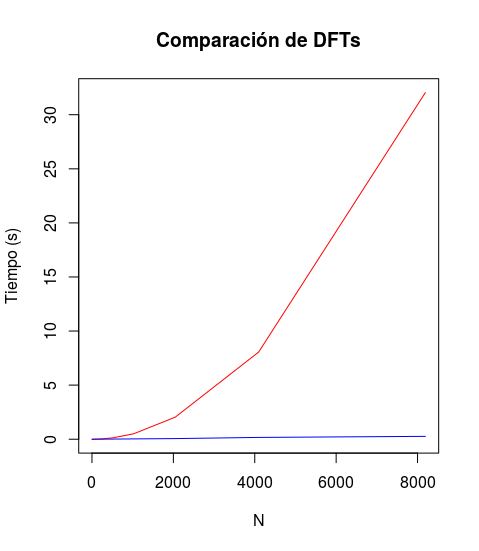
\includegraphics[width=0.5\textwidth]{images/dft_comp.png}
\caption{Comparación del tiempo de ejecución de las transformadas discretas en función de $N$. En rojo se muestra el algoritmo resultante de evaluar el polinomio asociado en las raíces de la unidad. En azul se muestra la transformada rápida recursiva.} \label{fig:nlogn_vs_n2}
\end{figure}

Este algoritmo suele recibir el nombre de Radix 2 DIT (Decimation in Time). Es posible mejorar el tiempo de ejecución de este algoritmo mediante distintas técnicas de programación, aunque todas estas versiones mantienen la complejidad $\Theta(N\log N)$. Los detalles se explican en \cite{cormen2009introduction}. Para concluir el análisis de este algoritmo, veamos algunas observaciones:

\begin{itemize}
    \item Notemos que los lemas \ref{lem:prop_cancel}, \ref{cor:prop_cancel} y \ref{lem:biseccion} son válidos igualmente para $\zeta_N$ y para $\zeta_N^{-1}$. Hasta ahora, para el cálculo de la transformada de Fourier hemos usado estas propiedades sobre $\zeta_N^{-1}$. Si ahora tenemos en cuenta que la transformada de Fourier inversa es esencialmente igual, utilizando $\zeta_N$ en vez de $\zeta_N^{-1}$ y multiplicando al final por la constante $1/N$, podemos construir un algoritmo análogo al Algoritmo \ref{alg:alg_fft_rec} para calcular la transformada de Fourier inversa, y también con complejidad $\Theta(N \log(N))$.
    
    \item Cuando $N$ no es una potencia de 2, es claro que no podemos utilizar este algoritmo. Sin embargo, en muchas ocasiones, no nos interesa el valor de la transformada de Fourier, sino operar con ella y después volver al espacio original aplicando la transformada inversa. Es por eso que, en estas situaciones, el algoritmo presentado sigue siendo de utilidad sin más que rellenar el vector sobre el que se va a aplicar la transformada con ceros hasta llegar a una potencia de 2. Veremos en la siguiente sección ejemplos de ello. Además, muchas de las aplicaciones de la transformada de Fourier son en campos como la teoría de la señal, o la computación cuántica, donde al trabajar en binario, los vectores a los que se suele aplicar son potencias de dos, de ahí la utilidad de este algoritmo. Aun así, introduciremos algunos algoritmos aplicables a otros tamaños de $N$.
\end{itemize}

Veamos en un ejemplo cómo funciona el Algoritmo \ref{alg:alg_fft_rec}.

\begin{ex}
    Retomamos el ejemplo \ref{ex:g_muchas_is}, en el que teníamos $g \equiv (1, i, -1, -i)$. Aplicamos el algoritmo. En primer lugar calculamos $g_0 = (1,-1)$ y $g_1 = (i,-i)$. Ahora, utilizamos la recursividad y aplicamos la FFT sobre $g_0$ y $g_1$.
    
    Para $g_0$, volvemos a dividir los coeficientes, obteniendo $g_{00} = (1)$ y $g_{01} = (-1)$. Como hemos llegado al caso $N = 1$ obtenemos inmediatamente que las transformadas de estos vectores son $y_{00} = 1$ e $y_{01} = -1$. Análogamente, sobre $g_1$ obtenemos que $y_{10} = i$ y $y_{11} = -i$.
    
    Una vez calculadas las transformadas de tamaño 1, podemos utilizarlas para calcular las transformadas $y_0 = (y_0(0),y_0(1))$ e $y_1 = (y_1(0),y_1(1))$. Para ello utilizamos la fórmula del Algoritmo \ref{alg:alg_fft_rec}.
    \begin{align*}
        y_0(0) &= y_{00}(0) + \zeta_2^0y_{01}(0) = 1 +(-1) = 0 \\
        y_0(1) &= y_{00}(0) - \zeta_2^0y_{01}(0) = 1 -(-1) = 2 \\
        \\
        y_1(0) &= y_{10}(0) + \zeta_2^0y_{11}(0) = i +(-i) = 0 \\
        y_1(1) &= y_{10}(0) - \zeta_2^0y_{11}(0) = i -(-i) = 2i
    \end{align*}
    Finalmente, una vez calculados $y_0 = (2,0)$ e $y_1 = (2i,0)$, podemos finalmente calcular la transformada de $g$, $y = (y(0),y(1),y(2),y(3))$.
    \begin{align*}
        y(0) &= y_0(0) + \zeta_4^0y_1(0) = 0 + 0 = 0 \\
        y(1) &= y_0(1) + \zeta_4^{-1}y_1(1) = 2 -i(2i) = 4 \\
        y(2) &= y_0(0) - \zeta_4^0y_1(0) = 0 - 0 = 0 \\
        y(3) &= y_0(1) - \zeta_4^{-1}y_1(1) = 2 +i(2i) = 0
    \end{align*}
    Hemos obtenido de nuevo que $Dg \equiv (0,4,0,0)$.
\end{ex}

\subsection{Convolución} \label{sec:fft:conv}

Sea $N \in \mathbb{N}$. Nos preguntamos cómo calcular la convolución de dos funciones $g,h \colon \mathbb{Z}_N \to \C$ a partir del algoritmo desarrollado en la sección anterior.  Utilizando el teorema de la convolución, podemos escribir la convolución en función de las transformadas de Fourier directa e inversa.
\[ g \ast h = D^{-1}(Dg \cdot Dh), \]
donde $\cdot$ denota al producto de Hadamard, esto es, el producto elemento a elemento en $\C^N$. Por tanto, el problema se reduce a aplicar $3$ transformadas de Fourier y $n$ productos. Si $N$ fuese una potencia de $2$, entonces cada transformada de Fourier conlleva $\theta(N \log N)$ operaciones, pero este puede no ser el caso. Para solucionarlo extendemos $g$ y $h$ como sigue. En primer lugar, consideramos $m \in \mathbb{N}$ tal que $2^{m-1} \ge N > 2^{m-2}$. Vamos a tomar $G, H \colon \mathbb{Z}_{M} \to \C$, donde $M = 2^m$, como
\[ G(n) = \begin{cases}
    g(n) & \text{si } n < N; \\
    0 & \text{en caso contrario.}
\end{cases} \quad H(n) = \begin{cases}
    h(n) & \text{si } n < N; \\
    h(n-M) & \text{si } M-N \le n < M; \\
    0 & \text{en caso contrario.}
\end{cases}\]
 Nótese que $H$ está bien definida, pues de $2N \le 2^m = M$ se deduce que $N \le M-N$, y $h(k) = H(k)$ para todo entero $k$ con $-N < k < N$. En consecuencia, tenemos que
\[(g \ast h)(n) = \sum_{k = 0}^{N-1} g(k) h(n-k) = \sum_{k = 0}^{M-1} G(k) H(n-k) = (G \ast H)(n)\]
para todo $n \in \{0, \ldots, N-1\}$. Por tanto, basta calcular $G \ast H$ para obtener $g \ast h$. Puesto que $G,H \in \mathbb{Z}_{2^m}$, se puede aplicar para calcular $G \ast H$ el método descrito anteriormente, cuya complejidad es $\theta(M \log M) = \theta(N \log N)$ ya que $N \le M \le 4N$ para cualquier valor de $N$. 

\subsubsection{Una aplicación: el producto de polinomios}

Sea $N \in \N$ y consideramos $P,Q\colon \mathbb{C} \to \mathbb{C}$ dos polinomios de grado menor que $N$. Podemos representarlos como $P(z) = \sum_{k=0}^{N-1}a_kz^k$ y $Q(z) = \sum_{k=0}^{N-1}b_kz^k$. Tenemos que el polinomio producto $PQ$ es un polinomio de grado menor que $2N-1$, y viene dado por
\[ PQ(z) = \sum_{k=0}^{N-1}\sum_{j=0}^{N-1}a_kb_jz^{k+j} = \sum_{n=0}^{2N-2}\sum_{k+j=n}a_kb_jz^n = \sum_{n=0}^{2N-2}\sum_{k=0}^{n}a_kb_{n-k}z^n.\]
Llamamos $c\colon \Z_{2N-1} \to \C$ a la función dada por $c(n) = \sum_{k=0}^{n}a_kb_{n-k}$. La imagen de $c$ es el vector de coeficientes del producto. Definimos los vectores de coeficientes extendidos $a\colon \mathbb{Z}_{2N-1} \to \C$ y $b\colon \Z_{2N-1} \to \C$ dados por $a(k)=a_k$ y $b(k)=b_k$ para cada $k \in \{0,\dots,N-1\}$, y $a(k) = b(k) = 0$ en caso contrario. Estos vectores verifican claramente que $P = P_a$ y $Q = P_b$, donde $P_a,P_b$ son los polinomios asociados a $a$ y $b$, respectivamente. Notemos que con esta definición se tiene, en particular, que $a(k)= 0$ para $N-1 < k < 2N-1$ y $b(n-k)=0$ para $-N < n-k < 0$. En consecuencia, si $n < k < 2N-1$, o bien $N < k < 2N-1$, o en caso contrario, $0 \le n < k < N$, de donde se deduce que $-N < -k < n-k < 0$. En cualquier caso, $a(k) b(n-k) = 0$. Por tanto, se tiene, para cada $n$ desde 0 hasta $2N-2$, que
\[ c(n) = \sum_{k=0}^{n}a_kb_{n-k} = \sum_{k=0}^{n}a(k)b(n-k) = \sum_{k=0}^{2N-2}a(k)b(n-k) = (a \ast b)(n).  \]
Esto es, el vector de los $2N-1$ coeficientes del polinomio producto se obtiene de convolucionar los coeficientes de los polinomios $P$ y $Q$, extendidos por ceros hasta dimensión $2N-1$. Tal y como vimos en el apartado anterior, si $M = 2N-1$, podemos construir un algoritmo basado en la transformada de Fourier rápida capaz de calcular este producto en $\Theta(M\log M) = \Theta(N\log N)$, lo que nos permite mejorar una vez más al algoritmo básico consistente en realizar las sumas del producto de coeficientes de uno en uno, para cada coeficiente del producto.



\subsection{Calculando transformadas rápidas para cualquier valor de $N$}

Supongamos que $N$ es cualquier natural. Vamos a reescribir la expresión de la transformada como una convolución, para poder aplicar los conocimientos adquiridos sobre el algoritmo de convolución para calcular una nueva transformada rápida. Este algoritmo se conoce como la transformada rápida de Bluestein y también es llamada \emph{Chirp-Z transform} \cite{rabiner1969chirp}.

Tomamos $N \in \N$ fijo y $\zeta = \zeta_N$. Partimos de la fórmula de la transformada discreta,
\[ Df(n) = \sum_{k=0}^{N-1} f(k) \zeta^{-kn}. \]
Multiplicamos por $\zeta^{n^2/2}$ a ambos lados, obteniendo
\[ \zeta^{n^2/2}Df(n) = \sum_{k=0}^{N-1}f(k)\zeta^{-kn+n^2/2} = \sum_{k=0}^{N-1}f(k)\zeta^{(2kn - n^2)/2}. \]
Notemos que se satisface la identidad $2kn -n^2 = -(n-k)^2 + k^2$. Sustituyendo en la expresión anterior, se tiene
\[ \zeta^{n^2/2}Df(n) = \sum_{k=0}^{N-1}f(k) \zeta^{((n-k)^2 - k^2)/2} = \sum_{k=0}^{N-1}f(k)\zeta^{-k^2/2}\zeta^{(n-k)^2/2}. \]
Por tanto,
\[ Df(n) = \zeta^{-n^2/2} \sum_{k=0}^{N-1}f(k) \zeta^{ - k^2/2}\zeta^{(n-k)^2/2} = \zeta^{-n^2/2}(g \ast h)(n), \]
donde $g(n) = f(n) \zeta^{-n^2/2}$ y $h(n) = \zeta^{n^2/2}$ para todo $n \in \{0, \ldots, N-1\}$. En consecuencia, para calcular $Df$ basta determinar la convolución de $g$ y $h$. En la Sección \ref{sec:fft:conv} vimos cómo calcular la convolución de forma eficiente a partir de la transformada rápida de Fourier presentada en la Sección \ref{sec:fft:fft}. Recordemos que este procedimiento es $\theta(N \log N)$. Por tanto, hemos dado con un algoritmo eficiente para calcular la DFT en el caso de que $N$ no sea una potencia de $2$. 

\begin{comment}
\text{No hay que escribir nada más! :)}

Definimos los vectores $b_n = f_n \overline{\zeta}^{\frac{1}{2}n^2}$, para $n = 0,\dots,N-1$, y $c_n = \overline{\zeta}^{\frac{1}{2}n^2}$, para $n = -(N+1),-N,\dots,-1,0,1,\dots,N+1$. Podemos expresar la igualdad anterior en términos de estos vectores como
\[ \overline{\zeta}^{-\frac{1}{2}n^2}Df(n) = \sum_{k=0}^{N-1}b_kc_{n-k} = (b \ast c)(n). \]

A partir de esta expresión es inmediato construir el algoritmo que se muestra en el algoritmo \ref{alg:alg_fft_bluestein}.

\begin{algorithm}
    \caption{Transformada de Fourier rápida (Bluestein)}
    \label{alg:alg_fft_bluestein}
    \begin{algorithmic}
        \REQUIRE $f = (f_0,\dots,f_{N-1})$, $N \in \N$.
        \FOR{ $n = 0,\dots,N-1$ }
            \STATE $b_n = f_n \overline{\zeta}^{\frac{1}{2}n^2} $
        \ENDFOR
        \FOR{ $n = -(N+1),-N,\dots,-1,0,1,\dots,N+1$}
            \STATE $c_n = \overline{\zeta}^{\frac{1}{2}n^2} $
        \ENDFOR
        \STATE \textbf{HELP: Extender por ceros}
        \STATE $\hat{b} = Db$ \COMMENT{Transformadas de tamaño potencia de 2}
        \STATE $\hat{c} = Dc$
        \STATE $\hat{d} = \hat{b}\hat{c}$
        \STATE $d = D^{-1}d$ \COMMENT{Aplicamos el teorema de convolución: $d = b \ast c$.}
        \FOR{$n=0,\dots,N-1$}
            \STATE $y_n = \zeta^{-\frac{1}{2}n^2}d_n$
        \ENDFOR
        \RETURN $y = (y_0,\dots,y_{N-1})$
    \end{algorithmic}
\end{algorithm}

Si nos fijamos, salvo las tres transformadas aplicadas, todas las operaciones consisten en, a lo sumo, recorrer $M$ elementos en un vector haciendo operaciones elementales en cada uno, donde $M$ es la potencia de 2 superior a $N$ más cercana. Por tanto, la complejidad de estas operaciones es de $\Theta(M)$. Por tanto, el peso del algoritmo está en las transformadas de Fourier que, en el apartado anterior, vimos cómo calcularlas con una complejidad $\Theta(M \log M)$. Es por tanto esta última de nuevo la complejidad del algoritmo.

\end{comment}

\subsection{Otras propuestas de FFT}

Para concluir la sección, vamos a ver brevemente otros algoritmos que tratan de calcular de forma eficiente la Transformada de Fourier Discreta. Por una parte, extenderemos las transformadas rápidas al caso multidimensional, y por otra parte comentaremos algunas ideas de transformadas rápidas propuestas para determinados valores de $N$.

\subsubsection{Transformada rápida bidimensional}

Sean $N_1, N_2 \in \N$ y $N = N_1N_2$. Recordemos que la transformada de Fourier discreta bidimensional de una función $f\colon \Z_{N_1} \times \Z_{N_2} \to \C$ viene dada por

\[ Df(n_1,n_2) = \sum_{k_1=0}^{N_1-1}\sum_{k_2=0}^{N_2-1}f(k_1,k_2)\zeta_{N_1}^{-n_1k_1}\zeta_{N_2}^{-n_2k_2} = \sum_{k_1=0}^{N_1-1}\left(\sum_{k_2=0}^{N_2-1}f(k_1,k_2)\zeta_{N_2}^{-n_2k_2}\right)\zeta_{N_1}^{-n_1k_1}. \]

Fijado $n_1 \in \{0,\dots,N_1-1\}$, llamamos $f_{n_1}\colon \Z_{N_2} \to \C$ a la función dada por $f_{n_1}(n_2) = f(n_1,n_2)$. Entonces, a partir de la expresión anterior, podemos expresar la transformada bidimensional en función de transformadas unidimensionales,

\[ Df(n_1,n_2) = \sum_{k_1=0}^{N_1-1}D_{N_2}f_{k_1}(n_2)\zeta_{N_1}^{-n_1k_1}. \]

Si, fijado $n_2 \in \{0,\dots,N_2-1\}$ llamamos $f^{n_2}_{*}\colon Z_{N_1} \to \C$ a la función discreta que tiene como imagen el vector $(D_{N_2}f_{0}(n_2),\dots,D_{N_2}f_{N_1-1}(n_2))$, entonces tenemos que
\[ Df(n_1,n_2) = \sum_{k_1=0}^{N_1-1}D_{N_2}f_{k_1}(n_2)\zeta_{N_1}^{-n_1k_1} = \sum_{k_1=0}^{N_1-1}f^{n_2}_{*}(k_1)\zeta_{N_1}^{-n_1k_1} = D_{N_1}f_{*}^{n_2}(n_1). \]

A partir de esta expresión podemos desarrollar una transformada de Fourier rápida a partir de las transformadas de Fourier rápidas de dimensión $N_1$ y $N_2$. En primer lugar, calculamos las $N_1$ transformadas rápidas de dimensión $N_2$, para las funciones $f_{n_1}$, $n_1 \in \{0,\dots,N_1-1\}$. Una vez calculadas, podemos construir las funciones $f^{n_2}_{*}$, $n_2 \in \{0,\dots,N_2-1\}$ y obtener el resultado final aplicándoles $N_2$ transformadas rápidas de dimensión $N_1$. Por tanto, la eficiencia de este algoritmo es de $N_1\Theta(N_2\log N_2) + N_2\Theta(N_1\log N_1) = \Theta(N_1N_2(\log N_1 + \log N_2)) = \Theta(N \log N)$. Cabe destacar que este procedimiento es generalizable para transformadas de dimensiones superiores. Los detalles pueden consultarse en \cite{cormen2009introduction}.

\subsubsection{Transformada rápida de Rader}

El algoritmo que vamos a ver a continuación está diseñado para usarse cuando la dimensión es un número primo, y se basa, como en el algoritmo de Bluestein, en el hecho de reescribir la transformada de Fourier como una convolución. Sea $p$ un natural primo. Sabemos que el anillo de enteros módulo $p$, denotado $\Z_p$, es un cuerpo, y que el grupo multiplicativo de sus unidades,  $\Z_p^{\cross} = Z_p \setminus \{0\} = \{1,2,\dots,p-1\}$, es un grupo cíclico. Es decir, existe $a \in \Z_p^{\cross}$ tal que para cualquier $k \in \{1,\dots,p-1\}$ existe un $l \in \{0,\dots,p-2\}$ tal que $a^l = n$ (en $Z_p$). Además, si $a$ es un generador, es claro que $a^{-1}$ es también un generador ya que ambos tienen el mismo orden.

Dados dos enteros $r$ y $q$ llamamos $R(r,q)$ al resto de dividir $r$ entre $q$. Supongamos que la clase de $a \in \{2, \ldots, p-1\}$ en $\Z_p^{\cross}$ genera $\Z_p^{\cross}$. Para cada $l \in \mathbb{N}$ escribimos $a^l = R(a^l,p) + n_l p$ para algún entero $n_l \in \Z$. Llamamos $\zeta = \zeta_p$. Obtenemos
\begin{align*}
    Df(n) &= \sum_{k=0}^{p-1} f(k) \zeta^{-kn} = f(0) + \sum_{l=0}^{p-2}f(R(a^l,p))\zeta^{-R(a^l,p) n} \\
          &= f(0) + \sum_{l=0}^{p-2}f(R(a^l,p))\zeta^{-(R(a^l,p) + n_l p)n} = f(0) + \sum_{l=0}^{p-2}f(R(a^l,p))\zeta^{-a^ln} .
\end{align*} 

Notemos que al cambiar a la variable $l$ hemos reordenado los sumandos, pero en ningún momento se ha modificado ninguno de los términos sumados. Si ahora tomamos $n \ne 0$ y reescribimos $n = R(a^m,p)$, obtenemos la expresión
\[ Df(R(a^m,p)) = f(0) + \sum_{l=0}^{p-2}f(R(a^l,p))\zeta^{-a^la^m} = f(0) + \sum_{l=0}^{p-2}f(R(a^{-(-l)},p))\zeta^{-a^{l+m}}. \]
Si ahora consideramos las funciones $g,h\colon \mathbb{Z}_{p-1} \to \C$ dadas por $g(k) = f(R(a^{-k},p))$ y $h(k) = \zeta^{-a^k}$, podemos reescribir la expresión como
\[ Df(R(a^m,p)) - f(0) = \sum_{l=0}^{p-2}h(l+m)g(-l) = \sum_{k=0}^{p-2}h(k)g(m-k) = (h \ast g)(m).\]

Es por tanto que, salvo el término $n = 0$, podemos reescribir la transformada de Fourier de dimensión prima como una convolución de vectores, y por tanto calcularla con el mismo orden de eficiencia que en el algoritmo previo. El caso que nos queda por calcular es aún más sencillo, puesto que, como ya hemos visto, $Df(0) = P_f(1) = f(0) + f(1) + \dots + f(p-1)$.

Aunque, a diferencia de la transformada de Bluestein, este algoritmo solo funciona para números primos, este suele ser más rápido, pues la convolución que se realiza es de dimensión $p-1$. Este número es siempre par (para $p > 2$), y en general suele ser altamente factorizable, lo que permite usarse en combinación con otros algoritmos, como Cooley-Tukey \cite{cooley}, que aceleran su funcionamiento. Para más información acerca de este algoritmo véase \cite{engelberg2017elementary}.

\subsubsection{Otras transformadas rápidas}

Hay que destacar también que los algoritmos de transformada rápida comentados no son los únicos. Al contrario, se conoce una gran cantidad de algoritmos que permiten calcular transformadas discretas de forma eficiente para determinados casos concretos y siguiendo técnicas particulares. De estos, además de los ya desarrollados, merece la pena mencionar la transformada rápida de Cooley-Tukey \cite{cooley}, que puede verse como una extensión de la transformada rápida recursiva, y se basa en la descomposición de la dimensión en factores no triviales, o la transformada rápida de Brunn \cite{bruun1978z}, un algoritmo diseñado para el caso en el que las funciones a transformar toman solo valores reales. La elección de unos algoritmos u otros a la hora de aplicar transformadas de Fourier vendrá determinada por la dimensión del problema y el comportamiento (precisión numérica y eficiencia) de los datos frente a los distintos algoritmos. 

\subsection{Comentarios finales}

En esta sección hemos visto cómo, además de todas las propiedades matemáticas interesantes presentes en la Transformada de Fourier Discreta, esta puede calcularse de manera eficiente, lo que permite a su vez agilizar otros procedimientos de gran utilidad en numerosos campos, como la convolución de funciones o el producto de polinomios que hemos comentado en esta sección, o algunas de las aplicaciones de las que hablaremos en las secciones posteriores. Es por ello que la Transformada de Fourier Discreta es de gran importancia en el mundo de la computación.

\begin{comment}

Rader's FFT algorithm - \url{https://en.wikipedia.org/wiki/Rader\%27s\_FFT\_algorithm}

\url{https://dsp.stackexchange.com/questions/15822/how-to-choose-a-fft-algorithm}

\end{comment}


%-----------------------------------------------------------------------------------------------------
%	ANDRÉS
%-----------------------------------------------------------------------------------------------------

\begin{comment}
\section{Aplicaciones en la teoría de algoritmos}

Richard Baraniuk - "FFTs are run billions of times a day"

Gilbert Strang - "FFT is the most important numerical algorithm of our lifetime"

\subsection{Convolución}

Determining optimal time translations!

Convolution neural networks!


\subsubsection{2D}

\subsection{Matrices circulares}

aplicaciones de las matrices circulares...

https://math.stackexchange.com/questions/2246941/book-recommendation-for-dft-fft

One important part of the discrete fourier transform is that it diagonalizes circulant operators (i.e. circular convolution). And circular convolution is related to linear convolution, which is what a linear time invariant system does (convolves its impulse response with the input). Thus, the basis provided by the DFT is a special one (it's not an arbitrary orthonromal basis).

Circular graphs...

Toeplitz and Circulant Matrices: A review

2012 - Matrix operations
\end{comment}

\newpage
\section{Quantum computing: Transformada de Fourier Cuántica} \label{sec:quantum}

La computación cuántica o quantum computing es sin duda alguna uno de los campos de investigación de moda en la informática teórica. No obstante, han pasado más de tres décadas desde que Richard Feynman, premio Nobel de física, propusiese utilizar la mecánica cuántica para diseñar un procesador que ampliase las posibilidades de la lógica binaria \cite{feynman}. El boom que ha sufrido la computación cuántica en la actualidad se debe a que los ordenadores cuánticos han dejado de ser un cuento de ficción para llegar al mundo real. En los últimos años varias empresas han apostado por el desarrollo de ordenadores cuánticos. Este es el caso de Google, Microsoft e IBM, donde trabajan los equipos de investigación Google Quantum A.I., Microsoft Quantum e IBM Q respectivamente. Los avances de estos grupos de investigación han sido impresionantes y han dado lugar a la creación de ordenadores cuánticos con hasta $20$ qubits \cite{quantum-lab, quantum-experimental, quantum-supremacy}. Se espera que la computación cuántica vea aplicaciones prácticas en unos $5$ años \cite{quantum-comercialize}. No obstante, habrá que esperar al menos $20$ años hasta que se comercialicen ordenadores cuánticos completamente funcionales \cite{quantum-manifesto}.

%encontrándonos actualmente en la barrera de resolver problemas mediante ordenadores cuánticos que no pueden resolverse por ordenadores tradicionales 

Un ejemplo de la importancia de los ordenadores cuánticos en la informática teórica es el Algoritmo de Shor \cite{shor}, que permite factorizar enteros en un ordenador cuántico en tiempo polinómico, esto es, realiza como mucho $p(n)$ operaciones, donde $p$ es un polinomio y $n$ es el número de bits del entero a factorizar. Este logro de la computación cuántica pone en duda la tesis fuerte de Church-Turing, que dice que cualquier modelo de cómputo físicamente realizable puede ser simulado por un ordenador clásico con, a lo sumo, un sobrecoste polinómico. En efecto, el problema de factorizar un entero ha sido uno de los más estudiados en la historia de la informática teórica pero el mejor algoritmo para computadores clásicos tiene complejidad $\theta\left(\exp(n^{1/3} \log^{2/3} n)\right)$, donde $n$ es el número de bits del entero a factorizar \cite[Capítulo 6]{primes}. Es por ello que factorizar un número se considera un problema imposible de resolver en un tiempo razonable mediante los ordenadores actuales cuando su número de bits es al menos $1024$. Esta es la razón por la cual la factorización de enteros juega un papel esencial en la criptografía moderna, siendo el fundamento del conocido criptosistema de clave pública RSA \cite{koblitz}. En consecuencia, si pudiésemos desarrollar un ordenador cuántico con la suficiente ``memoria'', entonces podríamos descifrar todas las conversaciones cifradas por RSA o algoritmos similares, que son los que se utilizan habitualmente en Internet. Éstas entre otras razones hicieron que Shor ganase el premio G\"odel en 1999 por la publicación de su algoritmo.

En esta sección introducimos el concepto de computación cuántica desde un punto de vista teórico, destacando el papel esencial que juega la Transformada de Fourier Discreta en el diseño de algoritmos cuánticos y, en particular, en el Algoritmo de Shor. Cabe destacar que el análisis de este algoritmo es bastante complejo. En consecuencia, nuestro objetivo es que el lector entienda la idea básica del algoritmo y pueda posteriormente consultar las múltiples referencias que se proporcionan.

\subsection{Una introducción a la mecánica cuántica y los qubits} \label{sec:qc:intro}

La mecánica cuántica surge con el fin de explicar aquellas cuestiones de la física en la que las teorías previas habían fracasado. Este es el caso del efecto fotoeléctrico. En este texto obviaremos el trasfondo físico de la mecánica cuántica y pasaremos directamente a resumir su formulación. No obstante, cabe destacar que los postulados de la mecánica cuántica son todavía un misterio para los físicos, como pone de manifiesto la siguiente cita de Richard Feynman:

`` La única diferencia entre un mundo regido por la probabilidad clásica y el mundo de la mecánica cuántica es que, por alguna razón, las probabilidades deberían ser negativas \cite{feynman}'' -- Richard Feynman. %premio Nobel de física en 1965.

Enunciamos a continuación los $4$ postulados de la mecánica cuántica. En la computación cuántica se asume que el tiempo es una variable discreta y, por tanto, introduciremos la mecánica cuántica bajo esta perspectiva. 
%En este texto consideramos que el tiempo es una variable discreta ya que ésta es la versión de la mecánica cuántica que se utiliza en la computación cuántica. 
Para mayor información sobre estos postulados véase \cite[Capítulo 2]{nielsen}. Junto con cada uno de los postulados desarrollaremos el concepto de qubit, que es la unidad básica de memoria usada en la computación cuántica.

El primer postulado de la mecánica cuántica determina las propiedades del objeto matemático bajo el cual se desarrolla la teoría.

\begin{postulate}[Espacio de estados] \label{post:1}
 Todo sistema físico aislado tiene asociado un espacio de Hilbert complejo y separable, que se denomina espacio de estados. En cada tiempo $t$ el sistema está completamente descrito por su \emph{vector de estado}, que es un vector unitario del espacio de estados, es decir, su norma es $1$. El sistema físico junto con su espacio de estados se denomina sistema cuántico.
\end{postulate}

En este punto hay que introducir la nomenclatura utilizada en la mecánica cuántica, que difiere de la usada en el álgebra lineal y el análisis funcional: 
\begin{enumerate}
    \item Los vectores de $H$ se escriben entre $\lvert$ y $\rangle$, esto es, $\ket{\Psi} \in H$, y se denominan \emph{kets}. 
    \item El vector dual de $\ket{\Psi}$ se denota $\bra{\Psi}$ y es conocido como \emph{bra}. 
    \item El producto escalar de dos vectores $\ket{\Psi}$ y $\ket{\varphi}$ se denota $\bra{\Psi}\ket{\varphi}$. 
    \item Dado un operador $A \in L(H,H)$, se denota por $A \ket{\Psi}$ a la imagen por $A$ del vector $\ket{\Psi}$. 
    \item Dado un operador $A \in L(H,H)$, se denota por $A^*$ a su operador adjunto. 
    \item Dado un operador$A \in L(H,H)$, se denota por $\bra{\Psi}A\ket{\varphi}$ al producto escalar entre $\ket{\Psi}$ y $A\ket{\varphi}$ o, equivalentemente, al producto escalar entre $A^*\ket{\Psi}$ y $\ket{\varphi}$.
    \item El producto tensorial de $\ket{\Psi}$ y $\ket{\varphi}$ se denota $\ket{\Psi} \otimes \ket{\varphi}$ o simplemente $\ket{\Psi} \ket{\varphi}$.
\end{enumerate}

En un estado cuántico arbitrario, se dice que una combinación lineal $\sum_{i} \alpha_i \ket{\Psi_i}$ es una \emph{superposición} de los estados $\ket{\Psi_i}$. Los números complejos $\alpha_i$ se denominan \emph{amplitudes}.

En la computación cuántica estamos interesados en el sistema cuántico conocido como \emph{qubit}, cuyo espacio de estados tiene dimensión $2$. Denotamos por $\{\ket{0}, \ket{1}\}$ a una base ortonormal de este espacio de estados. Siempre que trabajemos con un qubit utilizaremos una base ortonormal con esta nomenclatura. Los estados $\ket{0}$ y $\ket{1}$ se corresponden con los valores $0$ y $1$ de un bit en un computador clásico. No obstante, un qubit puede tomar muchos más valores. En efecto, un vector de estado de este sistema se puede escribir como $\ket{\Psi} = a \ket{0} + b \ket{1}$, donde $a,b \in \mathbb{C}$. Puesto que $\ket{\Psi}$ debe de ser unitario, obtenemos que $|a|^2 + |b|^2 = 1$. Según nuestra nomenclatura, $\ket{\Psi}$ es una superposición de los estados $\ket{0}$ y $\ket{1}$. Intuitivamente esto quiere decir que el sistema se encuentra en ambos estados al mismo tiempo, hecho que perdurará hasta que realicemos una medición. El lector puede entender en este punto la analogía con el famoso gato de Schrodinger.

El segundo postulado responde a cómo cambia o evoluciona un sistema cuántico %aislado 
con el tiempo. Recordemos previamente que un operador $U \in L(H,H)$ es unitario si es sobreyectivo e isométrico. Un operador es isométrico si preserva el producto escalar de $H$ o, equivalentemente, lleva vectores unitarios a vectores unitarios.
% Con aislado queremos decir que no está relacionado con ningún otro sistema cuántico. (?)

\begin{postulate}[Evolución] \label{post:2}
La evolución en el tiempo de un sistema cuántico aislado se describe mediante transformaciones lineales unitarias. Esto es, si $H$ es el espacio de estados del sistema, entonces el estado en el tiempo $t+1$ se calcula a partir del estado $\ket{\Psi}$ en el tiempo $t$ aplicando un operador unitario $U \in L(H, H)$ a $\ket{\Psi}$. Este operador solo depende de $t$.
\end{postulate}

Si el espacio de estados tiene dimensión finita, entonces los operadores unitarios coinciden con las isometrías.
%Recuérdese que, en vista de esta clasificación, una isometría 
Destacamos a continuación algunas isometrías que utilizaremos en el caso de los qubits. En primer lugar, la \emph{puerta NOT} es la isometría cuya matriz viene dada por
\[ X = \begin{pmatrix}
 0 & 1 \\ 1 & 0
\end{pmatrix}.\]
Nótese que $X \ket{0} = \ket{1}$ y $X \ket{1} = \ket{0}$, de ahí su nombre. La \emph{puerta de Hadamard} es la isometría cuya matriz viene dada por
\[ H = \frac{1}{\sqrt{2}}\begin{pmatrix}
 1 & 1 \\ 1 & -1
\end{pmatrix}.\]
Las puertas de cambio de fase dejan fijo a $\ket{0}$ y llevan $\ket{1}$ a $e^{i \theta} \ket{1}$ para cierto $\theta \in \mathbb{R}$. Esto es, la matriz de la isometría es
\[ R_\theta = \begin{pmatrix}
 1 & 0 \\ 0 & e^{i \theta}
\end{pmatrix}.\]

Como cabe de esperar, los sistemas cuánticos se pueden medir. El siguiente postulado determina cómo es el comportamiento de estos sistemas al realizar una medición.

\begin{postulate}[Medición] \label{post:3}
La medición de un sistema cuántico se describe por un conjunto de operadores $\{M_\lambda \in L(H,H) : \lambda \in \Lambda \}$, denominados operadores de medición, donde $\Lambda$ es el conjunto de todos los resultados posibles y $H$ el espacio de estados. Estos operadores verifican la igualdad 
\begin{equation} \label{eq:post3:operadores}
  \sum_{\lambda \in \Lambda} M_\lambda^* M_\lambda = I,
\end{equation}
donde $I$ es el operador identidad. La probabilidad de que al medir el sistema en un estado $\ket{\Psi}$ obtengamos el resultado $\lambda \in \Lambda$ viene dada por
\begin{equation} \label{eq:post3:prob}
  p(\lambda) = \bra{\Psi}M_\lambda^* M_\lambda \ket{\Psi},
\end{equation}
que pertenece a $[0,\infty]$. Es más, estos valores suman $1$ gracias a \eqref{eq:post3:operadores}, de ahí que se los denomine probabilidades. En efecto, tenemos que
\begin{equation*} \label{eq:post3:1}
  \sum\nolimits_{\lambda \in \Lambda} p(\lambda) = \sum\nolimits_{\lambda \in \Lambda} \bra{\Psi} M_\lambda^* M_\lambda \ket{\Psi} = \bra{\Psi} \sum\nolimits_{\lambda \in \Lambda} M_\lambda^* M_\lambda \ket{\Psi} = \bra{\Psi}\ket{\Psi} = 1.
\end{equation*}
Si $\lambda \in \Lambda$ es el resultado obtenido en la medición, entonces el estado del sistema cuántico pasa a ser el vector $M_\lambda \ket{\Psi}$ normalizado, esto es,
\begin{equation*} \label{eq:post3:estado}
 \frac{M_\lambda \ket{\Psi}}{\sqrt{\bra{\Psi}M_\lambda^* M_\lambda \ket{\Psi}}}.
\end{equation*}
\end{postulate}

En este texto nos centramos el la medición de qubits, que tiene dos posibles resultados, $0$ y $1$. Los operadores de medición vienen dados por las matrices
  \[ M_0 = 
     \left(
     \begin{matrix}
       1 & 0 \\
       0 & 0 \\
      \end{matrix} 
     \right)
     \text{ y }
     M_1 =
     \left(\begin{matrix}
       0 & 0 \\
       0 & 1 \\
     \end{matrix}
     \right).
  \]
  Supongamos que $\ket{\Psi} = a \ket{0} + b \ket{1}$ es el estado a medir. Entonces, la probabilidad de que el resultado sea $0$ viene dada por
  \[ p(0) =  \bra{\Psi} M_0^* M_0 \ket{\Psi} = \bra{\Psi} M_0 \ket{\Psi} = |a|^2. \]
  El estado del sistema en caso de que $0$ sea el resultado de la medición es
  \[ \frac{M_0 \ket{\Psi}}{|a|} = \frac{a}{|a|} \ket{0}.\]
  Análogamente, obtenemos que la probabilidad de que el resultado sea $1$ es $p(1) = |b|^2$ y, en caso de que se dé este resultado, el estado posterior es $b/|b| \ket{1}$.
  
  Desde el punto de vista del observador, dado $\theta \in \mathbb{R}$, los estados $\ket{\varphi} = e^{i \theta} \ket{\Psi}$ y $\ket{\Psi}$ son idénticos. En efecto, la probabilidad de que al medirlos el resultado sea $\lambda \in \Lambda$ es
  \[ \bra{\Psi}M_\lambda^* M_\lambda \ket{\Psi} = \bra{\Psi} e^{-i \theta} M_\lambda^* M_\lambda e^{i \theta} \ket{\Psi} = \bra{\varphi}M_\lambda^* M_\lambda \ket{\varphi}.\]
  Por tanto, podemos ignorar el factor $e^{i \theta}$, conocido como \emph{fase}, una vez hemos fijado una medición del sistema cuántico. En consecuencia, en el caso de un qubit, suponemos que los estados que siguen a una medición son $\ket{0}$ si el resultado fue $0$ y $\ket{1}$ en caso contrario. 

El último postulado describe cómo son los estados de un sistema cuántico que está compuesto por otros sistemas cuánticos conocidos.

\begin{postulate}[Sistemas compuestos]
El espacio de estados de un sistema cuántico compuesto es el producto tensorial de los espacios de estados de los sistemas cuánticos que lo componen. Además, si $\ket{\Psi_1}, \ldots, \ket{\Psi_n}$ eran los vectores de estado de estos sistemas cuánticos antes de componerse, entonces $\ket{\Psi_1} \otimes \cdots \otimes \ket{\Psi_n}$ fue el primer vector de estado del sistema cuántico compuesto. 
\end{postulate}


Recordemos en este punto que el producto tensorial $H_1 \otimes H_2$ de dos espacios de Hilbert separables $H_1$ y $H_2$ es un espacio de Hilbert separable. Es más, si $\{\ket{e_n} : n \in \mathbb{N}\}$ y $\{\ket{f_n}: n \in \mathbb{N}\}$ son dos bases ortonormales de $H_1$ y $H_2$, entonces $\{\ket{f_n}\ket{g_m} : n,m \in \mathbb{N}\}$ es una base ortonormal de $H_1 \otimes H_2$.

En la computación cuántica se trabaja con un sistema cuántico compuesto por qubits, denominado registro de qubits. El número de qubits que lo componen determinará la capacidad de cómputo del sistema. %se seleccionará a la hora de definir un algoritmo cuántico. 
Supongamos que este número es $n$. Entonces el espacio de estados es un espacio vectorial de dimensión $2^n$ y una base de este espacio es %está formada por los vectores que son productos tensoriales los elementos de las bases de los qubits: 
$\{\ket{x_1}\ket{x_2}\cdots\ket{x_n} : x_1, x_2, \ldots, x_n \in \{0,1\} \}$.
Para facilitar la escritura denotamos al vector $\ket{x_1}\ket{x_2}\ldots\ket{x_n}$ por $\ket{x_1 x_2 \ldots x_n}$, donde $x_1, \ldots, x_n \in \{0,1\}$. También utilizaremos la notación $\ket{j}$ con $j = x_n + x_{n-1}2 + \cdots + x_1 2^{n-1} \in \mathbb{N}$, esto es, $x_1 \ldots x_n$ es la representación en binario de $j$.

Los físicos han demostrado que en la práctica es posible controlar un registro de qubits, aunque el número $n$ de qubits que componen el sistema es todavía muy pequeño ($n \le 20)$. No obstante, un vector de estado de este sistema consta de $2^n$ coeficientes, cada uno de los cuales es un número complejo. Por tanto, $n$ qubits nos permiten almacenar una elevada cantidad de información, a diferencia de lo que sucede con los bits clásicos. Este hecho es una de las razones del potencial que presenta la computación cuántica. 

Los operadores unitarios de un registro de qubits son las isometrías de $\mathbb{Q}^{2^n}$. Sin embargo, también podemos aplicar isometrías a cualquier subconjunto de qubits del registro. En tal caso, los físicos han determinado que todo el sistema se ve afectado por esta operación. Concretamente, si la isometría $U$ afecta a $n-m$ qubits ($m < n$), entonces el estado del sistema completo es el resultado de aplicar $U \otimes I_{2^n}$ al vector de estado, donde $I_{2^n}$ la aplicación identidad actuando sobre el resto de qubits y $\otimes$ denota al producto de Kronecker de $U$ e $I_n$. 

\begin{ex}
Supongamos que tenemos $2$ qubits, queremos aplicar la puerta NOT al primer qubit. Si el estado del sistema cuántico es $(\ket{00} + \ket{11}) / \sqrt{2}$, entonces el siguiente estado del sistema completo será $(\ket{10} + \ket{01}) / \sqrt{2}$. Esto es, hemos aplicado la isometría
\[ X \otimes I_2 = \begin{pmatrix}
0 & 0 & 1 & 0 \\
0 & 0 & 0 & 1 \\
1 & 0 & 0 & 0 \\
0 & 1 & 0 & 0 \\
\end{pmatrix}.\]
Si a continuación aplicamos la puerta de Hadamard al segundo qubit obtendríamos el estado $(\ket{10} + \ket{11} + \ket{00} - \ket{01}) / \sqrt{4}$. Vemos que en la práctica la isometría afecta a cada una de las superposiciones que dan lugar al vector de estado, aplicándose ésta a los qubits sobre los que esté definida. Para más ejemplos e información sobre el uso del producto de Kronecker véase \cite[Capítulo 2]{nielsen}.
\end{ex}

Hasta el momento hemos estudiado puertas que actúan sobre un único qubit. El ejemplo más importante de puertas definidas sobre más de un qubit es  la puerta AND cuántica (también conocida como la puerta de Toffoli), que generaliza la puerta AND de la computación clásica. Esta puerta actúa sobre $3$ qubits extendiendo de forma lineal la aplicación $\ket{x}\ket{y}\ket{z} \mapsto \ket{x}\ket{y}\ket{z\oplus(x \land y)}$. En particular, cuando $z = 0$ esta puerta calcula en el tercer qubit el valor $x \land y$, de ahí el nombre. Viene dada por
\[ M_{\land} = \begin{pmatrix}
1 & 0 & 0 & 0 & 0 & 0 & 0 & 0\\
0 & 1 & 0 & 0 & 0 & 0 & 0 & 0\\
0 & 0 & 1 & 0 & 0 & 0 & 0 & 0\\
0 & 0 & 0 & 1 & 0 & 0 & 0 & 0\\
0 & 0 & 0 & 0 & 1 & 0 & 0 & 0\\
0 & 0 & 0 & 0 & 0 & 1 & 0 & 0\\
0 & 0 & 0 & 0 & 0 & 0 & 0 & 1\\
0 & 0 & 0 & 0 & 0 & 0 & 1 & 0\\
\end{pmatrix}.\]

Análogamente se pueden definir las puertas OR, NAND y NOR cuánticas.

Por último, hay que indicar cómo funciona la medición en el caso de los registros de qubits. Supongamos que $n$ es el número de qubits del registro. Cuando se mide el sistema completo cada qubit proporciona un resultado $x_j \in \{0,1\}$. La secuencia $x_1 \ldots x_n$ es el resultado del sistema completo. También nos referiremos a este resultado como el número natural $j = x_n + x_{n-1}2 + \cdots + x_1 2^{n-1}$. Es claro que hay $2^n$ resultados posibles. Si $\ket{\Psi} = \sum_{j = 0}^{N} a_j \ket{j}$ es el estado del registro, donde $N = 2^n$, entonces la probabilidad de que se de el resultado $j$ es $|a_j|^2$, en cuyo caso el resultado posterior es $a_j / |a_j| \ket{j}$. Este esquema de medición también responde al Postulado \ref{post:3}. 

En ocasiones nos interesa medir un número de qubits menor que $n$. Supongamos sin pérdida de generalidad que estos son los $m$ primeros $(m < n)$. En tal caso la probabilidad de que el resultado sea $x_1 \ldots x_m$ es la suma de las probabilidades de los resultados del sistema completo que comienzan por $x_1 \ldots x_m$. Además, si se da este resultado, entonces se eliminan del estado del registro los sumandos $a_j \ket{y_1 \ldots y_n}$ con $x_1 \ldots x_m \ne y_1 \ldots y_m$, normalizando el vector resultante. Este proceso es natural ya que el estado del registro solo puede ser superposición de aquellos resultados factibles.


Asumiendo estos axiomas podemos empezar a desarrollar matemáticas y, en particular, informática teórica. Si al lector le gustaría leer una descripción más intuitiva de los qubits recomendamos \cite[Capítulo 10]{algorithms}. 

%\begin{ex}
%  El sistema cuántico más sencillo es aquel cuyo espacio de estados $H$ es isomorfo a $\mathbb{C}$. Un vector de estado es de la forma $z \ket{\Psi}$, donde $\ket{\Psi}$ es el $1$ de $H$ y $z \in \mathbb{C}$ con $|z| = 1$. En este caso una isometría consiste en multiplicar por un número complejo de norma $1$. 
%\end{ex}

\subsection{Algoritmos cuánticos}

En esta sección definimos los algoritmos cuánticos, que es el modelo de computación utilizado por los ordenadores cuánticos. Intuitivamente, un ordenador cuántico consta de un registro de qubits sobre el que aplica una serie de operaciones unitarias. Posteriormente se mide el registro, devolviendo parte del resultado obtenido. Nótese que este resultado es aleatorio en el sentido de que distintas mediciones pueden dar lugar a distintos resultados. No obstante, la distribución de probabilidad de los resultados está fija siempre y cuando se apliquen los mismos operadores unitarios. Por tanto, con un número suficiente de repeticiones del proceso obtendremos el resultado deseado. %Por tanto, habrá un resultado más probable que otro. Teniendo esto en cuenta ya podemos definir los algoritmos cuánticos.

\begin{definition}
    Una operación cuántica es \emph{elemental} si actúa en $3$ o menos qubits del registro de qubits. A estas operaciones se las conoce como \emph{puertas cuánticas}.
\end{definition}

En la Sección \ref{sec:qc:intro} vimos múltiples ejemplos de puertas cuánticas (NOT, Hadamard, cambio de fase y AND). Denotaremos $\{0,1\}^n = \{x_1 x_2 \ldots x_n : x_i \in \{0,1\}\}$ y $\{0,1\}^* = \bigcup_{n = 0}^\infty \{0,1\}^n$.

\begin{definition}
    Sea $f \colon \{0,1\}^* \to \{0,1\}^q$ con $q \in \mathbb{N}$. Un algoritmo cuántico para calcular $f$ es un algoritmo clásico que, para cada $n \in \mathbb{N}$, describe $T(n)$ puertas cuánticas $G_1, \ldots, G_T$ de manera que para cada $x \in \{0,1\}^n$ podemos calcular $f(x)$ mediante el siguiente proceso con probabilidad mayor o igual que $2/3$:
    \begin{enumerate}
        \item Inicializamos un registro con $m$ qubits en el estado $\ket{x 0^{m-n}}$, donde $m \le T(n)$.
        \item Aplicamos de forma consecutiva las puertas cuánticas $F_1, \ldots, F_T$ al registro.
        \item Medimos el registro, obteniendo el valor $Y$.
        \item Devolvemos los $q$ primeros bits de $Y$.
    \end{enumerate}
    Decimos que el algoritmo cuántico tiene complejidad $\theta(T(n))$ y que la función $f$ es computable cuánticamente en tiempo $T(n)$.
\end{definition}

El valor $2/3$ presente en la definición es irrelevante. Esto es, si un algoritmo cuántico calcula $f$ con probabilidad $p \in ]0,1[$, entonces podemos repetirlo un determinado número de veces para conseguir calcular $f$ con probabilidad mayor o igual que $2/3$.

Todo algoritmo clásico se puede simular mediante uno cuántico de similar complejidad. En efecto, es ampliamente conocido que un algoritmo clásico se puede implementar mediante circuitos booleanos que utilizan las puertas NOT, AND y OR \cite[Capítulo 6]{arora}. Consecuentemente, podemos dar un algoritmo cuántico que simule este circuito usando las puertas cuánticas NOT, AND y OR \cite[Lema 10.10]{arora}.

El hecho de que la definición permita utilizar cualquier puerta que actúe sobre $3$ qubits puede ser un problema en la práctica ya que hay un número infinito de ellas. Recuérdese que en el caso de los circuitos booleanos solo se utilizan las puertas AND, OR y NOT ya que el resto se derivan de éstas. En el mundo cuántico nos encontramos un resultado similar, toda puerta cuántica se puede aproximar con la precisión que se desee mediante las puertas de Hadamard, AND y cambio de fase $R_{\pi /2}$ \cite[Teorema 10.12]{arora}. Es por ello que en la práctica basta con conseguir desarrollar estas tres puertas para construir un ordenador cuántico.

\begin{comment}
\begin{theorem}
 Para cada $d \ge 3$ y $\varepsilon > 0$, existe un entero positivo $l \le 100(d \log(1 / \varepsilon))$ tal que para cada matriz unitaria $U \in \mathcal{M}_{d\times d}(\mathbb{C})$ existen matrices $U_1, \dots, U_l \in \mathcal{M}_{d\times d}(\mathbb{C})$ con
 \[ ||U - U_1 \ldots U_l||_{\infty} < \varepsilon, \]
 donde $U_i$ consiste en aplicar la puerta de Hadamard, la puerta de Toffoli o la puerta de cambio de fase a $2$, $8$ o $2$ vectores de la base usual respectivamente.
\end{theorem}

Como consecuencia, en la práctica nos basta con construir ordenadores cuánticos solamente con las tres puertas usadas en el resultado. Además, se puede demostrar que, dado un algoritmo cuántico de complejidad $T(n)$, basta tomar $\varepsilon < 1 / (10 T(n))$ para que, a pesar del error cometido usando solo estas $3$ puertas, el algoritmo resultante calcule el mismo resultado que el original con probabilidad mayor que $1/2$ \cite[Teorema 10.12]{arora}.
\end{comment}

\subsection{La Transformada de Fourier Cuántica} \label{sec:quantum:qft}

La \emph{Transformada de Fourier Cuántica} es un algoritmo cuántico para calcular la Transformada de Fourier Discreta de un registro de qubits. Esto es, si el registro tiene $n$ qubits ($N = 2^n$) y su vector de estado es $\ket{f} = \sum_{j = 0}^{N-1} f(j) \ket{j}$, entonces la Transformada de Fourier Cuántica calcula el estado $\ket{Df} = \frac{1}{\sqrt{N}}\sum_{j = 0}^{N-1} Df(j) \ket{j}$, donde el factor $1/\sqrt{N}$ hace que la Transformada de Fourier Discreta sea una isometría sobre $\mathbb{C}^N$, como se demostró en el Corolario \ref{cor:isometria}.
%Recordemos que para cada $j \in \{0, \ldots, N-1\}$ se tiene que
%\[D f(j) = \frac{1}{\sqrt{N}} \sum_{k = 0}^{N-1} \zeta^{k j} f(k),\]
%donde $\zeta = \exp(-2 \pi i / N)$. 
%Puesto que $D$ es una isometría sobre $C^N$, la Transformada de Fourier Discreta es un operador válido en la computación cuántica. 

%En este punto nos proponemos encontrar un algoritmo cuántico para calcular la Transformada de Fourier Discreta que utilice el menor número posible de puertas elementales. 
Para entender este algoritmo cuántico recordemos que la Transformada de Fourier Discreta verifica la ecuación recurrente  \eqref{eq:rec_fft}, 
%Definimos la aplicación lineal de $C^N$ dada por $W_n \ket{j} = w^j \ket{j}$. Nótese que es una isometría. 
%En vista de \eqref{eq:dft:2} 
de donde deducimos que
\begin{equation} \label{eq:qft}
\begin{aligned}
    \ket{Df} & %= \sum_{j = 0}^{N-1} Df(j) \ket{j} 
     = \frac{1}{\sqrt{N}} \left(\sum_{j = 0}^{N/2} \left(Df_0(j) +  \zeta^j Df_1(j)\right) \ket{0} \ket{j} + 
     \sum_{j = 0}^{N/2} \left(Df_0(j)  -  \zeta^j Df_1(j)\right) \ket{1} \ket{j} \right). %\\
    %& = \ket{Df_0}\ket{0} + W_{n-1} \ket{Df_1}\ket{0} + \ket{Df_0}\ket{1} - W_{n-1} \ket{D f_1}\ket{1} 
    %& = \ket{0} (\ket{D f_0} + W_{n-1} \ket{D f_1}) + \ket{1} (\ket{D f_0} - W_{n-1} \ket{D f_1}).
\end{aligned}
\end{equation}
La Transformada de Fourier Cuántica consiste en utilizar de forma recursiva \eqref{eq:qft}. Para ello definimos la isometría de $C^N$ dada por $R_n \ket{j}\ket{0} = \ket{j}\ket{0}$ y $R_n \ket{j}\ket{1} = \zeta^j \ket{j}\ket{1}$ para todo $j \in \{0, \ldots, N/2-1\}$. Nótese que al aplicar $R_n$ a un registro arbitrario $\ket{\Psi} = \sum_{j = 0}^{N-1} a_j \ket{j}$ obtenemos
\begin{equation}
    R_n \ket{\Psi} = \sum_{j = 0}^{N/2-1} a_{2j} \ket{j}\ket{0} + \sum_{j = 0}^{N/2-1} \zeta^j a_{2j+1}  \ket{j}\ket{1}.
\end{equation}
Esta operación es justo la que nos faltaba para realizar la Transformada de Fourier Cuántica, que está descrita en el Algoritmo \ref{alg:qft}. 

\begin{table}[H]
    \centering
    \begin{tabular}{|L{0.9775\textwidth}|}
    \hline
    \multicolumn{1}{|c|}{\textbf{Transformada de Fourier cuántica}} \\
    \textbf{Entrada: } Un registro de $n$ qubits cuyo vector de estado es $\ket{f} = \sum_{j = 0}^{N-1} f(j) \ket{j}$. \\
    \textbf{Objetivo:} Aplicar la Transformada de Fourier Discreta para obtener $\ket{Df} = \sum_{j = 0}^{N-1} Df(j) \ket{j}$. \\
    \hline
    \end{tabular}   
    \begin{tabular}{|L{0.575\textwidth}|L{0.375\textwidth}|}
    \hline
    \textbf{Operación} & \textbf{Estado del registro} \\
    \hline
    \textbf{(1)} Notación: podemos escribir el registro usando $f_0$ y $f_1$. &
    \[\sum_{j = 0}^{N/2} f_0(j) \ket{j}\ket{0} + \sum_{j = 0}^{N/2} f_1(j) \ket{j}\ket{1}\] \\
    \hline
    \textbf{(2)} Aplicamos recursivamente a la Transformada de Fourier Cuántica a los $n-1$ qubits más significativos. &     
    \[\sum_{j = 0}^{N/2} Df_0(j) \ket{j}\ket{0} + \sum_{j = 0}^{N/2} Df_1(j) \ket{j}\ket{1}\] \\
    \hline
    \textbf{(3)} Aplicamos la isometría $R_{n}$. & 
    \[\sum_{j = 0}^{N/2} Df_0(j) \ket{j}\ket{0} + \sum_{j = 0}^{N/2} \zeta^j Df_1(j) \ket{j}\ket{1}\] \\
    \hline
    \textbf{(4)} Movemos el qubit menos significativo a la primera posición. &
    \[\sum_{j = 0}^{N/2} Df_0(j) \ket{0}\ket{j} + \sum_{j = 0}^{N/2} \zeta^j Df_1(j) \ket{1} \ket{j}\] \\
    \hline
    \textbf{(5)} Aplicamos la puerta de Hadamard al qubit más significativo. &  \[\ket{Df} = \sum_{j = 0}^{N-1} Df(j) \ket{j}\]
    \\
    \hline

    \end{tabular}
    \captionof{algorithm}{Transformada de Fourier cuántica.}
    \label{alg:qft}
\end{table}

El paso (5) de este algoritmo funciona correctamente gracias a \eqref{eq:qft}. No obstante, quedan varias cuestiones por resolver. En primer lugar, ¿cuántas puertas elementales se necesitan para aplicar $R_n$ en el paso (3)? La respuesta es $n-1$. En efecto, basta  utilizar $n-1$ puertas cambio de fase condicionadas al último qubit. Concretamente, la $j$-ésima puerta se aplica al $j$-ésimo y al último qubit y viene dada por
\[ \ket{x}\ket{y} \mapsto \begin{cases} \zeta^{2^{n-j-1}} \ket{x}\ket{y} & \text{si } x = y = 1;\\ \ket{x}\ket{y} & \text{en caso contrario.} \end{cases}  \]
El lector puede comprobar que la composición de estas puertas elementales es $R_n$. Por último, el paso (4) también se puede implementar con $n-1$ puertas elementales cuya función sea intercambiar dos qubits. En efecto, nótese que la permutación aplicada es composición de $n-1$ transposiciones.

En resumen, si $P(n)$ es el número total de puertas elementales aplicadas por el Algoritmo \ref{alg:qft} cuando trabaja sobre $n$ qubits, entonces se verifica la ecuación recurrente $P(n) = 2n-1 + P(n-1)$ y la condición inicial $P(0) = 1$. La solución de esta ecuación es $P(n) = n^2-1$. Concluimos el siguiente resultado.

\begin{lemma}[Transformada de Fourier cuántica]
  Existe un algoritmo cuántico tal que, para cada $n \in \mathbb{N}$, calcula la Transformada de Fourier Discreta de un registro con $n$ qubits utilizando $n^2-1 \in \theta(n^2)$ puertas elementales.
\end{lemma}

Consideramos un registro con $m$ qubits ($M = 2^m)$ cuyo estado es de la forma
\begin{equation} \label{eq:period}
  \ket{\Psi} = \frac{1}{\sqrt{K}}\sum_{j = 0}^{K-1} \ket{r_0 + j r},
\end{equation}
  donde $K = \lfloor (M-r_0) / r \rfloor$. La Transformada de Fourier Cuántica puede aplicarse a \eqref{eq:period} para calcular el periodo $r$. Esta propiedad es clave para el desarrollo del Algoritmo de Shor. Aplicando la Transformada de Fourier Cuántica a este registro obtenemos
  \begin{equation} \label{eq:qft:period}
  \ket{D \Psi} = \frac{1}{\sqrt{K M}} \sum_{j = 0}^M \left(\sum_{l = 0}^{K-1} \zeta^{(r_o + l r) j} \right) \ket{j}.
  \end{equation}
 El siguiente resultado determina una cota inferior de la probabilidad de obtener un múltiplo de $r$ al medir \eqref{eq:qft:period}, cuya demostración puede encontrarse en {\cite[Lemas 10.19 y 10.20]{arora}}.

\begin{theorem} \label{thm:qft}
  Existe $0 < c < 1$ tal que, para cualquier $m,r \in \mathbb{N}$ con $r < M = 2^m$, al medir \eqref{eq:qft:period} obtenemos, con probabilidad al menos $c/\log r$, un resultado de la forma $jr$ con $j \in \{0, \ldots, K-1\}$.
\end{theorem}
%Por tanto, es una aplicación lineal sobre $\mathbb{C}^{2^n}$ que, sobre la base ortonormal usual, viene dada por
%\[ \ket{k} \mapsto \frac{1}{\sqrt{2^n}} \sum_{j = 0}^{2^n-1} \zeta^{j k} \ket{j}, \]

\subsection{El Algoritmo de Shor}

En esta sección desarrollamos el Algoritmo de Shor para factorizar números en un ordenador cuántico. La Transformada de Fourier Cuántica jugará un papel esencial en este algoritmo.

\begin{remark} \label{rem:shor}
Nótese que para factorizar un número basta con diseñar un algoritmo que nos calcule, dado $N \in \mathbb{N}$, un divisor $x$ no trivial ($x \ne 0, N$) de $N$, que es lo que hace el Algoritmo de Shor. En efecto, podemos aplicar este algoritmo recursivamente a $x$ y $N/x$. Puesto que el número de factores primos (contando repetidos) de $N$ es a lo sumo $\log_2 N$, el número de veces que tenemos que aplicar recursivamente el Algoritmo de Shor para factorizar $N$ es $\log_2 N$ como mucho.
\end{remark}
%En consecuencia, si nuestro algoritmo para encontrar un divisor realiza $T(\log_2 N)$ pasos, entonces nuestro algoritmo para factorizar realiza $T(\log_2$

%Supongamos que nuestro algoritmo para encontrar un factor realiza $T(n)$ operaciones, donde $n$ es el número de bits de $N$. Entonces el algoritmo recursivo para factorizar $N$ realiza $R(n) = T(n) + R(\log_2(N/x)) + R(\log_2(x)) \le T(n) + 2 R(n-1)$....

El problema de calcular un divisor no trivial de $N$ se puede reducir al problema de encontrar raíces cuadradas no triviales de $1$ módulo $N$, que son aquellos enteros $x \in \{0, \ldots, N-1\}$ tales que $x \not \equiv \pm 1 \pmod{N}$ y $x^2 \equiv 1 \pmod{N}$. El término reducción es ampliamente utilizado en informática teórica y significa que podemos resolver el primer problema si conocemos la solución del segundo. El siguiente resultado pone de manifiesto la mencionada reducción.

\begin{lemma}
  Si $x$ es una raíz cuadrada no trivial de $1$ módulo $N$, entonces $\gcd(x+1, N)$ es un divisor no trivial de $N$. 
\end{lemma}
\begin{proof}
  Por hipótesis $N$ divide a $x^2 - 1 = (x-1)(x-1)$ pero $N$ no divide a $x-1$ ni a $x+1$. En consecuencia, $\gcd(x+1, N)$ debe de ser un divisor no trivial de $N$.
\end{proof}

El siguiente paso del Algoritmo de Shor es reducir el cálculo de una raíz cuadrada de $1$ módulo $N$ al cálculo del orden de cualquier elemento del grupo $\left(\mathbb{Z}/ N \mathbb{Z}\right)^{\times} = \{x \in \{0, \ldots, N-1\} : \gcd(x,N) = 1\}$. Recordemos que el orden de un elemento $x$ de un grupo finito es el menor número natural $r$ tal que $x^r = 1$. El Lema \ref{lem:reduccion-orden} efectúa esta reducción, que tiene probabilidad al menos $1/2$ de funcionar.

\begin{lemma} \label{lem:reduccion-orden}
  Sea $N$ un número entero con al menos dos factores primos distintos. Supongamos que escogemos aleatoriamente un entero $x \in \{0, \ldots, N-1\}$ primo relativo con $N$. Entonces, con probabilidad al menos $1/2$, el orden $r$ de $x \pmod{N}$ es par y $x^{r/2}$ es una raíz cuadrada no trivial de $1 \pmod{N}$.
\end{lemma}
\begin{proof}
  El resultado es una consecuencia del teorema de estructura del grupo multiplicativo de los enteros módulo $N$, que dice que  
  \begin{enumerate}
      \item  si $N = p_1^{e_1} \ldots p_t^{e_t}$ es la descomposición de $N$ en factores primos distintos, entonces  \[\left(\mathbb{Z}/ N \mathbb{Z}\right)^{\times} \equiv \left(\mathbb{Z}/ p_1^{e_1} \mathbb{Z}\right)^{\times} \times \cdots \times \left(\mathbb{Z}/ p_t^{e_t} \mathbb{Z}\right)^{\times};\]
      \item si $p$ es un primo distinto de $2$ y $e \ge 1$, entonces $\left(\mathbb{Z}/ p^{e} \mathbb{Z}\right)^{\times} = C_{\varphi(p^e)}$;
      \item si $e \ge 2$, entonces $\left(\mathbb{Z}/ 2^{e} \mathbb{Z}\right)^{\times} = C_2 \times C_{2^{e-2}}$.
  \end{enumerate}
  En efecto, utilizando este teorema podemos contar el número de elementos de $\left(\mathbb{Z}/ N \mathbb{Z}\right)^{\times}$ que son distintos de $-1$ y tienen orden par, siendo este número al menos $\varphi(N)/2$. 
\end{proof}

Resumiendo, hemos encontrado la siguiente reducción:

\begin{enumerate}
    \item \label{item:orden} Dado $x \in \left(\mathbb{Z} / N \mathbb{Z}\right)^\times$ aleatorio, calculamos el orden $r$ de $x$.
    \item Con probabilidad al menos $1/2$, $x^{r/2}$ es una raíz no trivial de $1$ módulo $N$.
    \item Con probabilidad al menos $1/2$, $\gcd(x^{r/2}+1, N)$ es un divisor no trivial de $N$.
\end{enumerate}
Si proporcionamos un algoritmo para el apartado \ref{item:orden}, entonces podemos calcular un divisor no trivial de $N$ repidiendo un número reducido de veces este proceso. Esta reducción ya se conocía antes de que surgiera el concepto de ordenador cuántico. No obstante, no se sabe resolver eficientemente el apartado \ref{item:orden} en un ordenador clásico. 

Fijado $x \in \left(\mathbb{Z} / N \mathbb{Z}\right)^\times$, consideramos la función $f(j) = x^j \pmod{N}$, que es periódica y su periodo es exactamente el orden $r$ de $x$. El problema de calcular $r$ se reduce pues a obtener el periodo de una función $f \colon \mathbb{N} \to \mathbb{Z}_N$. Los algoritmos clásicos necesitan evaluar $f$ en al menos $\sqrt{r}$ números naturales para calcular el periodo. Los ordenadores cuánticos nos permiten realizar todas estas evaluaciones a la vez mediante superposiciones de qubits. El Algoritmo \ref{alg:shor} muestra este procedimiento.

El paso (2) del Algoritmo \ref{alg:shor} se puede implementar mediante la conocida exponenciación rápida. La exponenciación rápida requiere $\theta(n^3)$ puertas lógicas en un circuito booleano \cite[Sección 5.3]{nielsen}. Esto implica que el paso (2) se puede realizar con $\theta(n^3)$ puertas elementales.

Como consecuencia del Teorema \ref{thm:qft}, el Algoritmo de Shor calcula el orden de $x$ módulo $N$ con probabilidad al menos $c / \log r$ para cierto $c > 0$ que no depende de $N$ ni de $x$. Repitiendo al menos $n$ veces el Algoritmo de Shor se obtiene una probabilidad 
\[1 - (c / \log_r)^n \ge 1 - e^{-c n / \log r} \ge 1-e^{-c} \] 
de obtener un múltiplo aleatorio de $r$. Para encontrar $r$ podemos repetir este algoritmo más veces y tomar el máximo común divisor de los resultados, que será probablemente $r$ pues la probabilidad de que dos enteros sean coprimos es $6 / \pi^2$. No obstante, esta solución está lejos de ser óptima. En la literatura hay mecanismos más eficientes para calcular $r$ que usan el Algoritmo \ref{alg:shor} y fracciones continuas. Si el lector quiere saber más al respecto puede leer \cite[Capítulo 5]{nielsen}, \cite[Capítulo 10]{arora} o la publicación original de Shor \cite{shor}. Estos mecanismos más eficientes permiten obtener el siguiente resultado.

\begin{theorem}[Algoritmo de Shor]
  El Algoritmo de Shor aplica $\theta(n^3)$ puertas elementales para calcular el orden de $x \in \left(\mathbb{Z}/N\mathbb{Z}\right)$, donde $n = \log_2 N$.
\end{theorem}

\begin{table}[H]
    \centering
    \begin{tabular}{|L{0.9775\textwidth}|}
    \hline
    \multicolumn{1}{|c|}{\textbf{Algoritmo de Shor}} \\
    \textbf{Entrada: } Dos naturales primos relativos $N$ y $x$ con $x < N$. \\
    \textbf{Objetivo:} Encontrar el menor entero positivo tal que $x^r = 1 \pmod{N}$. \\
    \hline
    \end{tabular}   
    \begin{tabular}{|L{0.9775\textwidth}|}
    \hline
    \textbf{Tamaño del registro:} $m + n$ qubits, donde $n = \lceil\log_2(N)\rceil$ y $m = 5 n$. \\  
    \textbf{Valor inicial del registro:} $\ket{0^m}\ket{0^n}$. \\
    \textbf{Notación:} $M = 2^m$. \\
    \hline
    \end{tabular}   
    \begin{tabular}{|L{0.575\textwidth}|L{0.375\textwidth}|}
    \hline
    \textbf{Operación} & \textbf{Estado del registro} \\
    \hline
    \textbf{(1)} Aplicamos la Transformada de Fourier Cuántica a los primeros $m$ qubits. &
    \[\frac{1}{\sqrt{M}} \sum_{j = 0}^{M-1} \ket{j}\ket{0^m}\] \\
    \hline
    \textbf{(2)} Aplicamos la transformación dada por
    $\ket{j}\ket{a} \mapsto a \oplus (x^j \pmod{N})$.
    & \[\frac{1}{\sqrt{M}} \sum_{j = 0}^{M-1} \ket{j}\ket{x^j \pmod{N}}\] \\
    \hline
    \textbf{(3)} Medimos los últimos $n$ qubits, obteniendo el valor $y_0$. & \[ \frac{r}{\sqrt{K}} \sum_{j = 0}^{K-1} \ket{r_0 + j r} \ket{y_0}, \] donde $K = \lfloor (M-r_0) / r\rfloor$ y $r_0$ es el primer número tal que $x^{r_0} = y_0$. \\
    \hline
    \textbf{(4)} Aplicamos la Transformada de Fourier Cuántica a los primeros $m$ qubits. & \[ \frac{1}{\sqrt{M K}}\sum_{j = 1}^M \left(\sum_{l = 0}^{K-1} \zeta^{(r_0+lr)j} \right) \ket{j} \ket{y_0}\] \\
    \hline
    \textbf{(5)} Medimos los primeros $m$ qubits, obteniendo un resultado $a$. Si $a$ de la forma $jr$, esto es, $x^{a} \equiv 1 \pmod{N}$, entonces devolvemos $a$. & \[\alpha \ket{a}\] \\
    \hline
    \end{tabular}
    \caption{Algoritmo de Shor para el cálculo de órdenes.}
    \label{alg:shor}
\end{table}

 Recordando  el Comentario \ref{rem:shor} concluimos el resultado principal de esta sección.

\begin{theorem}
  Existe un algoritmo cuántico para factorizar números enteros que utiliza como mucho $\theta(n^4)$ puertas elementales, donde $n = \log_2 N$.
\end{theorem}

En este punto hay que destacar que existen versiones del Algoritmo de Shor más eficientes. De hecho, la presentada por Shor utiliza $\theta(n^2 \log n \log \log n)$ puertas elementales \cite{shor}.


\newpage

%-----------------------------------------------------------------------------------------------------
%	MARINA
%-----------------------------------------------------------------------------------------------------

\section{Análisis de Fourier en el procesamiento del sonido} \label{sec:sonido}

Las señales musicales son generalmente mezclas de sonidos complejos con multitud de componentes sonoros distintos. Dada esta complejidad, la extracción de información relevante de una onda es un problema difícil. Un primer paso para una mejor comprensión de una señal dada es su descomposición en una construcción de bloques que son más accesibles de cara a los próximos pasos del procesamiento. En el caso de que esta construcción de bloques consista en un conjunto de funciones sinusoidales, entonces el proceso estará basado en Análisis de Fourier. En la música, y en el sonido en general, estas funciones tienen especial relevancia porque tienen un significado físico explícito en términos de la frecuencia. Como consecuencia el resultado de la descomposición descubre el espectro frecuencial de la señal, de la misma forma que un prisma separa la luz en su espectro de colores. La transformada de Fourier transformará una señal sonora que depende del tiempo en una representación que depende de la frecuencia.

\subsection{La Transformada de Fourier en el sonido}
%\subsection{Un primer acercamiento a la Transformada de Fourier en el sonido}

Tomemos, por ejemplo, la señal correspondiente al sonido de una única nota tocada al piano (véase la Figura \ref{fig:6.1}(a)). El tono de este sonido y su frecuencia fundamental están íntimamente relacionados. Asimismo, nos interesa determinar el contenido frecuencial de esta señal; para ello nos fijamos en las oscilaciones periódicas. Si ampliamos la señal hasta considerar sólo una sección de 10-ms (Figura \ref{fig:6.1}(b)) podemos observar que existe un comportamiento periódico en esta sección. De hecho, se pueden observar los tres picos principales de una señal sinusoidal (Figura \ref{fig:6.1}(c)). Entonces hay aproximadamente tres oscilaciones en una sección de 10-ms, lo que significa que esta señal contiene una componente frencuencial de unos 300Hz.

\begin{figure}[H]
\centering
    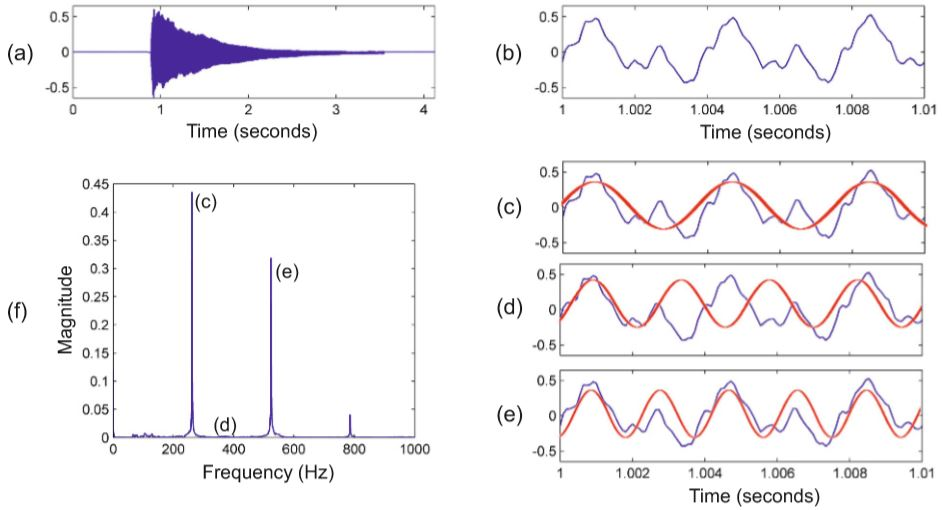
\includegraphics[width=0.85\textwidth]{images/81.jpeg}
    \caption{(a) Onda de la nota C4 (261.6Hz) tocada al piano- (b) Zoom a la sección de 10ms que comienza en $t=1$seg. (c-e) Comparación de la onda con sinusoides de varias frecuencias $\omega$. (f) Coeficientes de magnitud $d_\omega$ en función de las distintas frecuencias $\omega$ \cite[Capítulo 2]{muller2015fundamentals}.}
  \label{fig:6.1}
\end{figure}

Aquí, la principal idea del análisis de Fourier es comparar la señal dada con sinusoides de varias frecuencias $\omega\in\mathbb{R}$ (medidas en Hz). Como resultado obtenemos, para cada $\omega$ considerada, un coeficiente de magnitud $d_{\omega}\in\mathbb{R}\geq0$ y un coeficiente de fase $\varphi_{\omega}\in\mathbb{R}$ (del que hablaremos más tarde). Si el valor de $d_{\omega}$ es grande, existirá una gran similaridad entre la señal y el sinusoide de frecuencia $\omega$, y la señal contendrá una oscilación periódica a esa frecuencia (Figura \ref{fig:6.1}(c)). En el caso de que $d_{\omega}$ sea pequeña, entonces la señal no contendrá una componente periódica a esa frecuencia (Figura \ref{fig:6.1}(d)). Si representamos gráficamente los coeficientes $d_{\omega}$ sobre varios parámetros de frecuencia $\omega\in\mathbb{R}$ (Figura \ref{fig:6.1}(f)) podemos observar que el mayor valor se alcanza en la frecuencia $\omega=$ 262 Hz, aproximadamente, que es la frecuencia que se corresponde con el tono $p =$ 60, es decir, la nota C4 (Do). De hecho, esta es la nota tocada al piano de nuestro ejemplo inicial.


\subsubsection{Transformada de Fourier en señales analógicas}

Una onda de sonido, o una señal en general, se representa como una función $f:\mathbb{R\rightarrow R} $ que asigna a cada instante $t\in\mathbb{R}$ el valor de la amplitud de la onda $f(t)\in\mathbb{R}$. Si consideramos una señal analógica, tanto el tiempo como la amplitud son parámetros reales y continuos. Así, diremos que una señal analógica es periódica con periodo $\lambda$ si $f$ es periódica de periodo $\lambda$.

\subsubsection{El papel de la fase $\varphi$}

Un tipo de señal analógica periódica importante es el sinusoide.
\begin{definition}
    Un sinusoide es una función $g:\mathbb{R\rightarrow R} $ definida como
        \begin{equation}\label{eq:Asinusoid}
            g(t):=A \sin(2\pi(\omega t-\varphi))
        \end{equation}
    para $t\in\mathbb{R}$. El parámetro $A$ se denomina amplitud, cuya intepretación física se corresponde con el volumen del sonido. El parámetro $\omega$ es la frecuencia (medida en Hz), que se corresponde con el tono del sonido. El parámetro $\varphi$ es la fase (medida en radianes), que indica la posición relativa de una oscilación en su ciclo. El periodo del sinusoide es $\lambda=1/\omega$.
\end{definition}

 Se considerarán aquellas oscilaciones que están normalizadas respecto a su energía media considerando $A=\sqrt{2}$. Así, para cada frecuencia $\omega$ y fase $\varphi$ dadas  obtenemos el sinusoide $\cos_{\omega,\varphi}:\mathbb{R\rightarrow R}$ dado por
\begin{equation}\label{eq:sinusoid}
\cos_{\omega,\varphi}:=\sqrt{2}\cos(2\pi(\omega t-\varphi))
\end{equation}
para $t\in\mathbb{R}$. Dada la periodicidad del coseno, el dominio del parámetro $\varphi$ es $[0,1)$. 
\begin{definition}
    Dadas dos señales analógicas $f$ y $g$, la superposición de ambas señales se expresa como $f+g$ y está definida como la suma punto a punto
    \begin{equation}
        (f+g)(t):=f(t)+g(t).
    \end{equation}
    De forma similar, la escala de la señal $f$ de factor $a\in\mathbb{R}$ se expresa como $af$ y está definida como:
    \begin{equation}
        (af)(t):=af(t).
    \end{equation}
\end{definition}

Cuando medimos el grado de coincidencia entre el sinusoide de frecuencia $\omega$ y una señal dada, contamos con la libertad de poder trasladar el sinusoide en el tiempo. Este grado de libertad se expresa a través del parámetro de la fase $\varphi$. Como se ilustra en la Figura \ref{fig:6.2}, el grado de similaridad entre la señal de frecuencia dada y el sinusoide depende en gran medida de la fase. Para entender ésto en profundidad, formalicemos cómo se comparan la señal y el sinusoide.

\begin{figure}[H]
\centering
    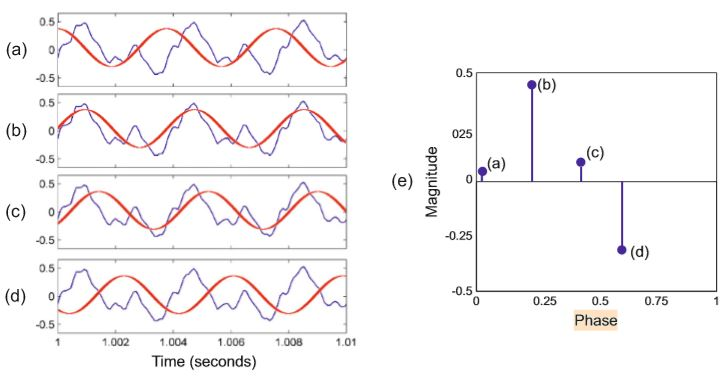
\includegraphics[width=0.85\textwidth]{images/82.jpeg}
    \caption{(a-d) Señal a frecuencia fijada $\omega=$ 262 Hz comparada con sinusoides con diferentes fases $\varphi\in\{0.05,0.24,0.45,0.6\}$. (e) Valores que expresan el grado de mislaridad entre la señal y los cuatro sinusoides de diferentes fases \cite[Capítulo 2]{muller2015fundamentals}.}
  \label{fig:6.2}
\end{figure}

\subsubsection{Midiendo el grado de similaridad}

Sean $f:\mathbb{R}\rightarrow\mathbb{R}$ y $g:\mathbb{R}\rightarrow\mathbb{R}$. El grado de similaridad de ambas funciones podría basarse en si su comportamiento es similar a lo largo del tiempo: por ejemplo, podríamos decir que ambas funciones son similares si su signo es igual en cada intervalo de tiempo. Este comportamiento se puede capturar en forma de integral del producto de ambas funciones, esto es,
\begin{equation}\label{eq:similarity}
\int_{t\in\mathbb{R}}f(t)g(t)dt.
\end{equation}
Así, si $f$ y $g$ son ambas positivas o ambas negativas la mayor parte del tiempo, el producto será positivo y el valor de la integral será grande. En caso contrario, su valor será pequeño.
\newline
Basándonos en la medida de similaridad \eqref{eq:similarity} podemos comparar la señal original dada con frecuencia $\omega$ fija y el sinusoide $\cos_{\omega,\varphi}$ definido en \eqref{eq:sinusoid}. Así, podemos definir formalmente el coeficiente de magnitud y el coeficiente de fase:
\begin{equation}\label{eq:magnitude}
d_{\omega}:=\max_{\varphi\in[0,1)}\left(\int_{t\in\mathbb{R}}f(t)\cos_{\omega,\varphi}(t)\diff t\right),
\end{equation}
\begin{equation}\label{eq:phase}
\varphi_{\omega}:=\argmax_{\varphi\in[0,1)}\left(\int_{t\in\mathbb{R}}f(t)\cos_{\omega,\varphi}(t)\diff t\right).
\end{equation}
Como se dijo anteriormente, $d_\omega$ nos indica la intensidad de la frecuencia $\omega$ en la señal dada, y la fase $\varphi_\omega\in[0,1)$ nos indica cuánto es necesario que desplacemos el sinusoide de frecuencia $\omega$ a lo largo del tiempo para conseguir una mejor aproximación del mismo a la señal original.

\subsubsection{La transformada de Fourier}

Utilizaremos el siguiente lema.

\begin{lemma} \label{lem:complex_exp}Sean $z\in\mathbb{C}$ y $\theta\in[0,1)$ tal que $z=\abs{z}\exp(2\pi i\theta)$. Entonces:
\begin{itemize}
    \item $\abs{z}=\max_{\varphi\in[0,1)}\{x\cos(2\pi\varphi)+y\sin(2\pi\varphi)\}$;
    \item $\theta=\argmax_{\varphi\in[0,1)}\{x\cos(2\pi\varphi)+y\sin(2\pi\varphi)\}$.
\end{itemize}
\end{lemma}

\begin{proof} Escribimos $z = x + i y$ con $x,y \in \R$. Para cualquier $\varphi \in [0,1)$, denotando $a = \cos{2\pi\varphi}$ y $b = \sin{2\pi\varphi}$, se tiene que
\[\left(ax+by\right)^2 = a^2 x^2 + 2 b x a y + b^2 y ^2 \le a^2 x^2 + b^2 x^2 + a^2 y^2 + b^2 y^2 = x^2 + y^2,\]
donde se ha usado la desigualdad $(bx)(ay) \le (b^2x^2 + a^2y^2)/2$. Nótese que $\cos{2\pi \theta}=x/\sqrt{x^2+y^2}$ y $\sin{2\pi\theta}=y/\sqrt{x^2+y^2}$. Se obtiene pues la igualdad
\[x\cos{2\pi\varphi}+y\sin{2\pi\varphi}=\sqrt{x^2+y^2}=\abs{z},\]
concluyendo la demostración.
\end{proof}

\begin{corollary}
Sea $c_{\omega}:=(d_\omega/\sqrt{2})\exp(2\pi i(-\varphi_\omega))$. Entonces $\hat{f}(\omega)=c_{\omega}$.
\end{corollary}
\begin{proof} Usando la fórmula del coseno de la suma en $\cos_{\omega,\varphi}(t)$ obtenemos que 
\[\frac{d_\omega}{\sqrt{2}}=\max_{\varphi\in[0,1)}\left\{\cos(2\pi\varphi)\int_{t\in\mathbb{R}}f(t)\cos(2\pi\omega t)\diff t + \sin(2\pi\varphi)\int_{t\in\mathbb{R}}f(t)\sin(2\pi\omega t)\diff t\right\}.\]
Aplicando el Lema \ref{lem:complex_exp} deducimos que
\begin{equation*}\label{eq:fhat}
    \hat{f}(\omega)
    = \int_{t\in\mathbb{R}}f(t)\cos(2\pi\omega t)\diff t + i\int_{t\in\mathbb{R}}f(t)\sin(2\pi\omega t)\diff t = c_{\omega}. \qedhere
\end{equation*}
\end{proof}

La idea básica en lo que sigue es expresar $\hat{f}(\omega)$ como coordenadas polares, obteniendo 
%y ponerlas en común en un único coeficiente complejo, $c_{\omega}$. En particular, $d_\omega$ y $\varphi_\omega$ se pueden expresar en términos de $\hat{f}(\omega)$ usando la expresión de $c_{\omega}$:
\begin{equation}
    d_\omega=\sqrt{2}\abs{\hat{f}(\omega)}, \quad  \varphi_\omega=-\gamma_\omega/2\pi,
\end{equation}
donde $\abs{\hat{f}(\omega)}$ y $\gamma_\omega$ son las coordenadas polares de $\hat{f}(\omega)$.


\subsubsection{Representación de Fourier de la señal}

La señal original $f$ puede ser reconstruida partiendo de su transformada. En principio, la reconstrucción es directa: se superponen los sinusoides de todas las frecuencias posible $\omega\in\mathbb{R}$, cada uno con peso del respectivo coeficiente $d_\omega$ y trasladado según el respectivo $\varphi_\omega$. Ambos tipos de información se recogen en el coeficiente complejo $c_\omega$. En el caso de una señal analógica, estamos tratando con parámetros de frecuencia continuos, donde la superposición se convierte en una integral sobre el espacio paramétrico, de forma que la reconstrucción de la señal viene dada por

\begin{equation} \label{eq:f}
    f(t) =\int_{\omega\in\mathbb{R}_\geq{0}}d_\omega\sqrt{2}\cos(2\pi(\omega t-\varphi_\omega))\diff \omega
         =\int_{\omega\in\mathbb{R}}c_\omega\exp(2\pi i\omega t)\diff \omega.
\end{equation}

Nótese que la fórmula \eqref{eq:fhat} para la transformada de Fourier y la fórmula \eqref{eq:f} para la representación de Fourier de la señal son casi idénticas. La principal diferencia es que los parámetros temporal y frecuencial están intercambiados. Esta relación se estudiará más a fondo al final de la sección.

\subsection{Señales digitales}

Cuando se usa tecnología digital, sólo un número finito de parámetros puede ser almacenado y procesado. Por eso es necesario convertir las señales analógicas en representaciones finitas. Este proceso se denomina digitalización. Así, distinguiremos entre dos tipos de señales: las analógicas y las digitales.

\subsubsection{Digitalización}
Algunas señales analógicas como los sinusoides están ya caracterizados por un pequeño número de parámetros que pueden usarse para representar la señal de forma discreta, pero para las señales analógicas en general son necesarias otras formas de modelado que nos permitan llegar a una representación con un número finito de parámetros. Las dos formas más comunes de digitalización de señales de audio son el sampleado (o muestreo) y la cuantización.

El sampleado se refiere al proceso de reducir una señal continua en el tiempo (señal-CT) a una señal discreta en el tiempo (señal-DT). Uno de los pasos que se aplican en esta conversión es el llamado sampleado equidistante. Dada una señal analógica $f:\mathbb{R}\rightarrow\mathbb{C}$ y un número positivo real $T\textgreater 0$, se construye la función $x:\mathbb{Z}\rightarrow\mathbb{C}$ definida como

\begin{equation}\label{eq:DT}
    x(n):=f(nT)
\end{equation}

El valor $x(n)$ se conoce como muestra tomada en el tiempo $t=nT$ de la señal analógica original $f$. Este procedimiento también es conocido como $T$-sampling, donde $T$ es el periodo de muestreo. Su inversa $F_s:=1/T$ es conocida como el ratio de muestreo, que especifica el número de muestras por segundo y se mide en Hz.
En la Figura \ref{fig:6.3}(a) se muestra un ejemplo donde la señal-DT se representa con puntos rojos. Esta señal cuenta con 13 muestras en los primeros dos segundos. Así, el ratio de muestreo $F_s=$6.5Hz y el periodo de muestreo $T$=0.154seg.

En general, el procedimiento de muestreo implica una pérdida de información en el sentido de que, generalmente, una señal analógica original no puede ser reconstruida partiendo de su versión sampleada. El proceso de sampleado causa efectos como el aliasing, donde ciertos componentes de frecuencias de la señal se hacen indistinguibles. Existen condiciones bajo las que esta reconstrucción sí es posible.

\begin{theorem}
  Si la señal analógica original $f$ no contiene frecuencias mayores que 
  \begin{equation}
      \Omega:=F_s/2=1/(2T)Hz,
  \end{equation} 
  entonces $f$ puede ser reconstruida perfectamente a partir de su versión sampleada $x$. En este caso se dice que $f$ es una señal $\Omega$-limitada, donde $\Omega$ es conocida como la frecuencia Nyquist.
\end{theorem}

La demostración detallada y las aplicaciones varias de este teorema pueden encontrarse, entre otros, en \cite[Capítulo 2]{muller2015fundamentals}, \cite[Capítulo 4]{proakis1996digital}

\begin{figure}[H]
\centering
    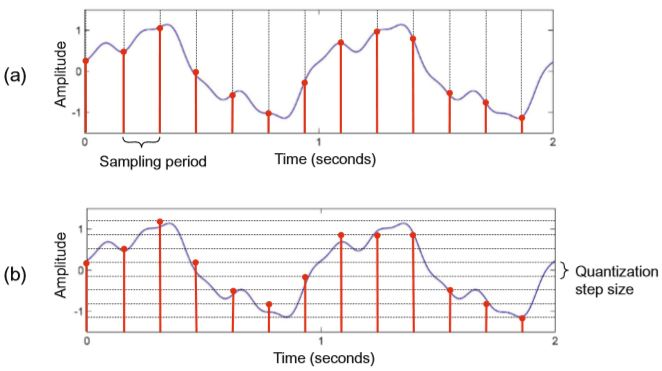
\includegraphics[width=0.60\textwidth]{images/83.jpeg}
    \caption{Proceso de digitalización de una señal analógica (curva continua en azul) a una señal digital (puntos rojos). (a) Sampleado. (b) Cuantización. \cite[Capítulo 2]{muller2015fundamentals}}
  \label{fig:6.3}
\end{figure}

Tras el muestreo o sampLleado de la señal analógica, el segundo paso para alcanzar la digitalización de la misma es reemplazar el rango continuo de las posibles amplitudes de la señal, contenido en $\mathbb{C}$, por un rango discreto de posibles valores, contenido en un conjunto discreto $\Gamma\in\mathbb{C}$. Este proceso es conocido como cuantización. Este proceso es modelado por una función $Q:\mathbb{C}\rightarrow\Gamma$, conocida como cuantizador. Muchos de los cuantizadores usados suelen simplemente redondear o truncar el valor de la señal analógica a alguna unidad de precisión. Por ejemplo, un cuantizador uniforme común con un tamaño de paso $\Delta$ puede ser definido como
\begin{equation}
    Q(a):=\mathrm{signo}(a)\Delta\Bigl\lfloor\frac{\abs{a}}{\Delta}+\frac{1}{2}\Bigr\rfloor
\end{equation}
donde $\lfloor·\rfloor$ indica el truncamiento del número real contenido al mayor entero por debajo de este número. Notar que, en el caso de $\Delta$=1, el cuantizador $Q$ simplemente redondea al entero más cercano. Al igual que el muestreo, la cuantización generalmente implica pérdida de información ya que valores diferentes de la señal analógica pueden ser aplicados al mismo valor digitall. La diferencia entre el valor de la señal analógica original y el valor cuantizado recibe el nombre de error de cuantización, que puede minimizarse reduciedo $\Delta$, lo que a su vez implica que el número de valores cuantizados aumente. La Figura \ref{fig:6.3}(b) muestra el resultado de samplear y cuantizar una señal analógica con $\Delta$=1/3, lo que da lugar a 8 valores cuantizados de la señal.


\subsubsection{Espacio de señales digitales}

En lo que sigue usaremos $x$ e $y$ para denotar las señales-DT, $x\colon \mathbb{Z}\rightarrow\mathbb{C}$ e $y \colon \mathbb{Z}\rightarrow\mathbb{C}$. Para el parámetro temporal, donde normalmente se usa $t$ en las señales-CT, usaremos $t_k$ para las señales-DT.

\begin{definition}
    Dada una señal-DT $x:\mathbb{Z}\rightarrow\mathbb{C}$, se define la energía de $x$, y se nota $E(x)$, como:
    \begin{equation*}
        E(x):=\sum_{k\in\mathbb{Z}}\abs{x(t_k)}^2.
    \end{equation*}
\end{definition}
Así, el espacio $\ell^2(\mathbb{Z})$ puede verse contenido en el espacio de las señales-DT y puede redefinirse como
\begin{equation*}
    \ell^2(\mathbb{Z}):=\{x\colon \mathbb{Z}\rightarrow\mathbb{C} \text{ tal que } E(x)\textless\infty\}.
\end{equation*}
Obviamente no todas las señales-DT tienen energía finita. Por ejemplo, el sinusoide sampleado $x$ dado por $x(t_k)=\sin{\pi k/16}$ no es de cuadrado sumable. Por otro lado, cualquier señal-DT con un número finito de valores no nulos tiene energía finita. Así, el espacio $\mathbb{C}^N$ para $N\in\mathbb{N}$ arbitrario puede verse como un subespacio de $\ell^2(\mathbb{Z})$ extendiendo el vector $x=(x(t_0),x(t_1),...,x(t_{N-1}))^T\in\mathbb{C}^N$ a una señal $x(t_k)$ que es 0 para $k\textless0$ y $k\geq{N}$.

\subsubsection{Transformada de Fourier en señales digitales}
Sea $x\in\ell^2(\mathbb{Z})$ una señal-DT arbitraria de energía finita. Entonces su representación de Fourier es:

\begin{equation}
    x(t_k)=\int_{\omega\in[0,1)}c_\omega\exp_\omega(k)\diff \omega
\end{equation}

donde $\exp_\omega(k)=\exp(2\pi i\omega k)$, para $k\in\mathbb{Z}$. Además, los coeficientes $c_\omega$ vienen dados por la transformada de Fourier de $x$, $\hat{x} \colon [0,1)\rightarrow\mathbb{C}$, dada por

\begin{equation}\label{eq:FT-DT}
    c_\omega=\hat{x}(\omega):=\sum_{k\in\mathbb{Z}}x(t_k)\overline{\exp_\omega(k)}.
\end{equation}

\subsubsection{Transformada discreta de Fourier en señales digitales}

Sea $x\in\ell^2(\mathbb{Z})$ una señal-DT. Asumimos que la energía de $x$ está concentrada en el intervalo $[0, N-1]$ de forma que $x(t_k)\approx$ 0 para $k\in\mathbb{Z}\backslash[0, N-1]$. Entonces de \eqref{eq:FT-DT} obtenemos:

\begin{equation}\label{eq:TF-DT-N}
    \hat{x}(\omega)=\sum_{k\in\mathbb{Z}}x(t_k)\overline{\exp_\omega(k)}\approx\sum_{k=0}^{N-1}x(t_k)\overline{\exp_\omega(k)}
\end{equation}

para cada frecuencia $\omega$. Puesto que $\hat{x}$ es 1-periódica, sólo es necesario considerar las frecuencias $\omega\in[0,1)$. En la práctica, la transformada de Fourier se suele computar únicamente para un subconjunto finito de frecuencias. En particular, fijando un número $M\in\mathbb{N}$, se consideran las frecuencias $\omega=m/M$ donde $m\in[0,M-1]$, que se corresponde con un proceso de 1/$M$-sampling del espacio frecuencial $[0,1)$. Aunque el número $N$ de puntos temporales y el número $M$ de frecuencias consideradas son independientes, es conveniente asumir $N=M$. Esta consideración es la que permitirá la formulación matricial de la Transformada de Fourier Discreta explicada en la Sección \ref{sec:matrix}.

En lo que sigue asumiremos por tanto $N=M$. Además, $x\in\ell^2(\mathbb{Z})$ será cero fuera del intervalo $[0,N-1]$, de forma que tendremos la igualdad en \eqref{eq:TF-DT-N}. Este tipo de señales-DT son también conocidas como señales de longitud finita, donde $N$ es la longitud de la señal. Además, no son necesarias todas las frecuencias $\omega\in[0,1)$ para caracterizar la señal de longitud $N$. De hecho el teorema de inversión \ref{thm:inv} nos asegura que las frecuencias $n/N$ para $n\in[0,N-1]$ son suficientes para representar dicha señal. Este hecho nos permite llegar a la expresión de la transformada discreta de Fourier de la señal-DT $x$, dada por
\begin{equation}\label{eq:TFD-DT}
    Dx(t_k)=\hat{x}(n/N)=\sum_{k=0}^{N-1}x(t_k)\overline{\exp_{n/N}(k)}=\sum_{k=0}^{N-1}x(t_k)\zeta^{-nk},
\end{equation}
donde, recordemos, $\zeta=\exp(2\pi i/N)$.

\subsubsection*{Interpretación de la transformada discreta de Fourier en señales digitales}

Para una correcta interpretación de la transformada discreta de Fourier en señales digitales conviene estudiar el caso particular de la aproximación de Riemann aplicada a la transformación de señales analógicas a digitales. Sea $f$ una señal-CT y $x$ su versión T-sampleada. Entonces:

\begin{equation}
    \begin{split}
        \hat{x}(\omega) &= \sum_{k\in\mathbb{Z}}x(t_k)\exp(-2\pi i\omega k) \\
        & = \sum_{k\in\mathbb{Z}}f(t_kT)\exp(-2\pi i\omega k) \\
        & \approx \int_{t\in\mathbb{R}}f(tT)\exp(-2\pi i\omega t)\diff t \\
        & = \frac{1}{T}\int_{t\in\mathbb{R}}f(t)\exp(-2\pi i\omega t/T)\diff t \\
        & = \frac{1}{T}\hat{f}(\omega/T), 
    \end{split}
\end{equation}

donde se ha usado la regla de sustitución para integrales indefinidas al reemplazar $tT$ por $t$.\newline
Entonces, ¿cuál es la relación de los coeficientes de la transformada discreta de Fourier con la señal analógica $f$ original?

\begin{equation}\label{eq:DT-CT-approx}
    Dx(t_k) \approx \hat{x}(n/N) \approx \frac{1}{T}\hat{f}(n/NT)
\end{equation}

Esta aproximación ha de estudiarse con cuidado. La primera aproximación sólo es buena si las muestras de $x(t_k)$ son cercanas a cero fuera del intervalo $[0, N-1]$. Esta condición se corresponde con la de que la señal analógica original $f$ sea cercana a cero fuera del intervalo $[0,(N-1)/T]$. La segunda aproximación sólo es buena si $f$ no contiene componentes frecuenciales que superen la frecuencia Nyquist $1/(2T)$Hz. Además, para valores grandes de $n$ (frecuencias altas de las funciones exponenciales) la aproximación empeora. Además, si asumimos que $f$ es una señal real se tiene que $\hat{f}(\omega)=\overline{\hat{f}(-\omega)}$, $\hat{x}(\omega)=\overline{\hat{x}(-\omega)}$ y $Dx(t_k)=\overline{Dx(t_{N-k})}$. Se deduce entonces que los coeficientes de la transformada discreta de Fourier son redundantes para $k=\lfloor N/2\rfloor+1,\dots,N-1$.

\begin{figure}[H]
\centering
    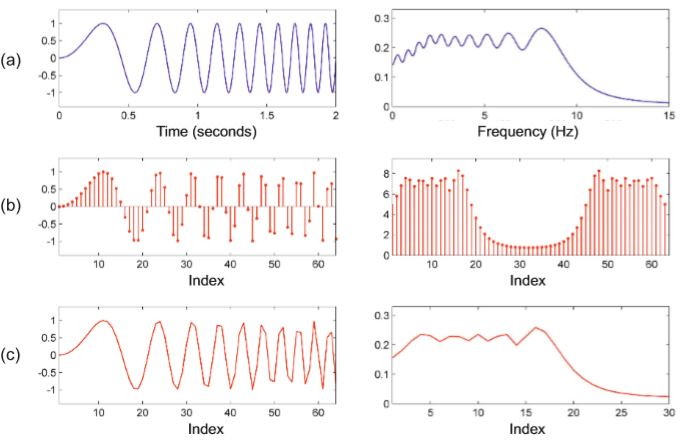
\includegraphics[width=0.75\textwidth]{images/84.jpeg}
    \caption{Aproximación mediante la transformada discreta de Fourier. (a) Señal analógica y su transformada de Fourier. (b) Señal digitalizada a $T=$1/32 y coeficientes de la transformada discreta a $N=$64. (c) Interpolación de la señal digitalizada y los coeficientes de la transformada discreta. \cite[Capítulo 2]{muller2015fundamentals}}
  \label{fig:6.4}
\end{figure}

Como ejemplo, consideremos la señal analógica de la figura \ref{fig:6.4}(a), donde se asume que la señal es cero fuera del intervalo considerado $[0,2]$. La transformada de Fourier se muestra para frecuencias $\omega\in[0,15]$. Tras digitalizar la señal usando un ratio de muestreo $F_s=$32Hz, obtenemos una señal de longitud finita $N=$64. Aplicando la transformada discreta de Fourier, obtenemos los valores que se muestran en \ref{fig:6.4}(b). Aplicando ahora la aproximación \eqref{eq:DT-CT-approx}, obtenemos $Dx(t_k)/32\approx\hat{f}(n/2)$. Así, por ejemplo, $t_30$ se corresponde con la frecuencia $\omega=$15Hz (ver figura \ref{fig:6.4}(c)). La resolución frecuencial resultante es de 0.5Hz.


%-----------------------------------------------------------------------------------------------------
%	BIBLIOGRAFÍA
%-----------------------------------------------------------------------------------------------------
\newpage
\printbibliography
%\nocite{*}

\end{document}
